%%%%%%%%%%%%%%%%%%%%%%%%%%%%%%%%%%%%%%%%%%%%%%%%%%%%%%%%%%%%%%%%%%%%%%%%%%%

\documentclass[a4paper,oneside,12pt]{article}
\usepackage{mystyle}

\begin{document}

\title{\Large\bf Linear regression}
\author{%%
  Minh Van Nguyen \\
  \url{mvngu@gmx.com}
}
\date{\today}
\maketitle


%%%%%%%%%%%%%%%%%%%%%%%%%%%%%%%%%%%%%%%%%%%%%%%%%%%%%%%%%%%%%%%%%%%%%%%%%%%

\section{The mean}
\label{sec:mean}

The goal of this document is to use statistics for prediction.  You
will learn about a statistical model called \emph{linear regression}.
Before doing so, you need to know how to calculate the \emph{mean} of
a bunch of numbers.

Let's start with an example.  Consider the following sequence of
numbers:
%%
\begin{equation}
\label{eqn:Hong_Kong_teenagers_heights}
\begin{matrix}
167, & 181, & 176, & 173, & 172, & 174, & 177, & 177, & 172, & 169.
\end{matrix}
\end{equation}
%%
These numbers are the heights~(in centimetres) of ten Hong Kong
teenagers.\footnote{
  Data are from the following website:
  \url{http://web.archive.org/web/20180428184006/http://wiki.stat.ucla.edu/socr/index.php/SOCR_Data_Dinov_020108_HeightsWeights},
  accessed 2018-04-28.
}
To calculate the mean of the numbers
in~\eqref{eqn:Hong_Kong_teenagers_heights}, first you add the numbers
together to get the total
\[
167 + 181 + 176 + 173 + 172 + 174 + 177 + 177 + 172 + 169
=
1738.
\]
Next, divide the total by how many numbers are in the sequence.  There
are ten numbers in~\eqref{eqn:Hong_Kong_teenagers_heights} so you
divide the total by ten to get
\[
173.8
=
\frac{1738}{10}.
\]
This tells you that the ten heights
in~\eqref{eqn:Hong_Kong_teenagers_heights} has a mean of $173.8$
centimetres.

The mean of a bunch of numbers is also called the \emph{average}.
However, the word average can have three different meanings in the
context of statistics.  When someone talks about the average of a
bunch of numbers, the person might be talking about one of three
things: the mean, median, or mode of the numbers.  So when you use the
word average, you must be careful about the sense in which you use the
word.  However, when you use the word mean, there is little confusion
about what you have in mind.  From the above example, the mean of a
bunch of numbers can be defined as follows:

\begin{definition}
\textbf{Mean.}
Let $\seq{a_1}{a_2}{a_n}$ be a sequence of $n$ numbers.  The
\emph{mean} of the sequence is defined as the number
\[
\frac{
  \sum_{i=1}^n a_i
}{
  n
}
=
\frac{
  \sumseq{a_1}{a_2}{a_n}
}{
  n
}.
\]
The mean of the sequence $\seq{a_1}{a_2}{a_n}$ is written as $\abar$.
\end{definition}

Each of $\seq{a_1}{a_2}{a_n}$ is a number, where $a_1$ is the first
number in the sequence, $a_2$ is the second number, and so on, with
$a_n$ being the $n$-th number.  Going back to
\List{eqn:Hong_Kong_teenagers_heights}, you see that the first number
is $a_1 = 167$, the second number is $a_2 = 181$, the third is
$a_3 = 176$, and so on, with the tenth number being $a_{10} = 169$.
The list has ten numbers so you have $n = 10$.  The sigma notation
$\sum_{i=1}^n a_i$ means that you add together all numbers in the
sequence $\seq{a_1}{a_2}{a_n}$ from $i = 1$ to $i = n$.  This is the
same as writing
\[
\sum_{i=1}^n a_i
=
\sumseq{a_1}{a_2}{a_n}.
\]
If you have a sequence of one hundred numbers and you want to write
the sum of the numbers, it is easier to use the sigma
notation~(i.e.~the symbol $\sum$) to denote the sum than it is to
write out all the one hundred numbers.

\begin{example}
Use the sigma notation to write the sum of the first five Fibonacci
numbers.  Calculate the actual sum and the mean of the five numbers.
\end{example}

\begin{solution}
The Fibonacci numbers are numbers in the sequence
\[
\begin{matrix}
0, & 1, & 1, & 2, & 3, & 5, & 8, & 13, & 21, \dots
\end{matrix}
\]
The Fibonacci numbers go on forever.  The numbers form an infinite
sequence.  The first number in the sequence is $a_1 = 0$, the second
number is $a_2 = 1$, the third is $a_3 = 1$, the fourth is $a_4 = 2$,
and the fifth is $a_5 = 3$.  The sum of the first five numbers in the
Fibonacci sequence can be written as $\sum_{i=1}^5 a_i$.  The actual
sum of those five numbers is
%%
\begin{align*}
\sum_{i=1}^5 a_i
&=
\sumseq{a_1}{a_2}{a_5} \\[4pt]
&=
0 + 1 + 1 + 2 + 3 \\[4pt]
&=
7.
\end{align*}
%%
The mean of the five numbers is
\[
\abar
=
\frac{
  \sum_{i=1}^5 a_i
}{
  5
}
=
\frac{7}{5}
\]
which is $1.4 = 7 / 5$.
\end{solution}

\begin{exercise}
Consider the first $12$ positive integers.
%%
\begin{packedenum}
\item\label{subex:sigma_first_12_positive_integers}
  Use the sigma notation to write the sum of the first $12$ positive
  integers.

\item\label{subex:sum_first_12_positive_integers}
  Calculate the sum of the first $12$ positive integers.

\item\label{subex:mean_first_12_positive_integers}
  Calculate the mean of the first $12$ positive integers.
\end{packedenum}
\end{exercise}
%%
\ifbool{showSolution}{
\begin{solution}
\solutionpart{subex:sigma_first_12_positive_integers}
The first $12$ positive integers are $\seq{1}{2}{12}$.  The first
number is $a_1 = 1$, the second is $a_2 = 2$, and so on, with the
$12$-th number being $a_{12} = 12$.  The sum of the $12$ integers can
be written as $\sum_{i=1}^{12} a_i = \sum_{i=1}^{12} i$.

\solutionpart{subex:sum_first_12_positive_integers}
The sum of the $12$ integers is
%%
\begin{align*}
\sum_{i=1}^{12} a_i
&=
\sumseq{1}{2}{12} \\[4pt]
&=
78.
\end{align*}

\solutionpart{subex:mean_first_12_positive_integers}
The mean of the $12$ integers is
%%
\begin{align*}
\frac{
  \sum_{i=1}^{12} a_i
}{
  12
}
&=
\frac{
  \sumseq{1}{2}{12}
}{
  12
} \\[4pt]
&=
\frac{78}{12} \\[4pt]
&=
\frac{13}{2}
\end{align*}
%%
which is $\abar = 6.5 = 13 / 2$.
\end{solution}
}{}

\begin{table}[!htbp]
\centering
\begin{tabular}{lc}         \toprule
Day       & Hours studying \\\midrule
Monday    & $3$            \\[6pt]
Tuesday   & $3.5$          \\[6pt]
Wednesday & $4$            \\[6pt]
Thursday  & $2.5$          \\[6pt]
Friday    & $4$            \\[6pt]
Saturday  & $4$            \\[6pt]
Sunday    & $4$            \\\bottomrule
\end{tabular}

\caption{%%
  The number of hours that a student spent on studying for each day of
  a week.  The studying hours are during the evening of the given day.
}
\label{tab:study_hours}
\end{table}

\begin{exercise}
\Table{tab:study_hours} shows the number of hours that a student spent
on studying during the evening.  For the particular week in the table,
calculate the mean number of hours that the student spent studying
during the evening.
\end{exercise}
%%
\ifbool{showSolution}{
\begin{solution}
Let $x_i$ be the number of hours spent studying during the evening of
day $i$.  If $i = 1$, the first day is Monday.  If $i = 2$, the second
day is Tuesday.  And so on.  The sum of the hours spent studying is
%%
\begin{align*}
\sum_{i=1}^7 x_i
&=
3 + 3.5 + 4 + 2.5 + 4 + 4 + 4 \\[4pt]
&=
25.
\end{align*}
%%
As there are seven numbers, the mean is $\xbar = 25 / 7 \approx 3.57$,
rounded to two decimal places.  That is, during a particular week the
student spent an average of $3.57$ hours studying during the evening.
\end{solution}
}{}


%%%%%%%%%%%%%%%%%%%%%%%%%%%%%%%%%%%%%%%%%%%%%%%%%%%%%%%%%%%%%%%%%%%%%%%%%%%

\section{Scatter plot}

A \emph{scatter plot} is a graph of a given data set.  The data set is
usually in the form of a table of values and the scatter plot is a
visual representation of the data in the table.  In many cases, it is
easier to understand a table of values if the data in the table are
represented as a scatter plot.  For example, \Table{tab:height_weight}
shows the height versus weight of ten Hong Kong teenagers; the data
are from \Section{sec:mean}.  Looking at the data in the table, it can
be difficult to make sense of what is going on.  Suppose you graph the
data as the scatter plot in \Figure{fig:height_weight_scatterplot}.
Now it is easier to understand what is going on.  For one, the scatter
plot in \Figure{fig:height_weight_scatterplot} shows that, generally
speaking, the taller is a Hong Kong teenager the heavier that the
person weighs.  A scatter plot allows you to see general trends in the
data that are not apparent from what is presented in a table of
values.

\begin{table}[!htbp]
\centering
\begin{tabular}{cc} \toprule
Height & Weight \\\midrule
$167$  & $51$   \\
$181$  & $61$   \\
$176$  & $69$   \\
$173$  & $64$   \\
$172$  & $65$   \\
$174$  & $55$   \\
$177$  & $64$   \\
$177$  & $61$   \\
$172$  & $50$   \\
$169$  & $54$   \\\bottomrule
\end{tabular}

\caption{%%
  The height and weight of ten Hong Kong teenagers.  Height is
  measured in centimetres and weight is measured in kilograms.
}
\label{tab:height_weight}
\end{table}

\begin{figure}[!htbp]
\centering
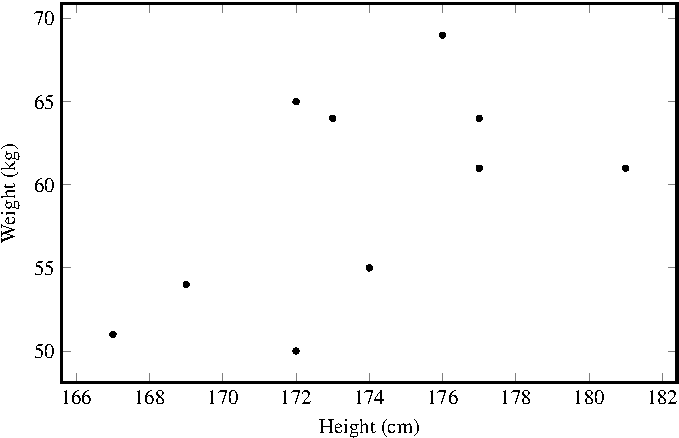
\includegraphics[scale=1.1]{image/07/height-weight-scatterplot.pdf}
\caption{%%
  A scatter plot of the height versus weight of ten Hong Kong
  teenagers.  The data are from \Table{tab:height_weight}.
}
\label{fig:height_weight_scatterplot}
\end{figure}

\begin{table}[!htbp]
\centering
\begin{tabular}{ccc}                    \toprule
Student & Hours studying & Test score \\\midrule
1       & $4$            & $5$        \\
2       & $3$            & $5$        \\
3       & $6$            & $7$        \\
4       & $2$            & $4$        \\
5       & $1$            & $2$        \\
6       & $5$            & $7$        \\
7       & $8$            & $9$        \\
8       & $9$            & $10$       \\
9       & $4$            & $6$        \\
10      & $10$           & $10$       \\
11      & $7$            & $9$        \\\bottomrule
\end{tabular}

\caption{%%
  The number of hours that eleven students spent on studying for a
  test versus their test scores.  The test is marked out of ten.
}
\label{tab:test_score}
\end{table}

\begin{exercise}
\Table{tab:test_score} shows how many hours that students spent on
studying for a test and their test scores.  Graph the data in the
table as a scatter plot.  What can you conclude from the scatter plot?
\end{exercise}
%%
\ifbool{showSolution}{
\begin{solution}
\Figure{fig:test_score} shows a scatter plot of the data from
\Table{tab:test_score}.  The scatter plot shows that the more time a
student spent on studying for a test, the higher is the student's test
score.

\begin{figure}[!htbp]
\centering
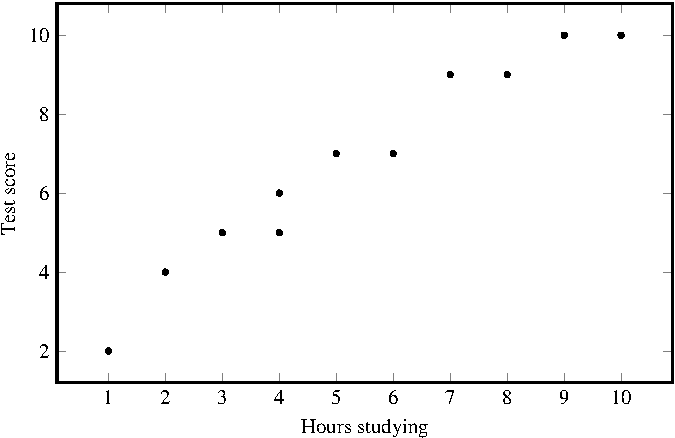
\includegraphics[scale=1.1]{image/07/test-score-scatterplot.pdf}
\caption{%%
  The number of hours that students spent studying for a test versus
  their test scores.  The data are from \Table{tab:test_score}.
}
\label{fig:test_score}
\end{figure}
\end{solution}
}{}


%%%%%%%%%%%%%%%%%%%%%%%%%%%%%%%%%%%%%%%%%%%%%%%%%%%%%%%%%%%%%%%%%%%%%%%%%%%

\section{Linear regression}

The basic idea of linear regression is to fit a straight line to a
data set.  The idea is best explained through a detailed example.


%%%%%%%%%%%%%%%%%%%%%%%%%%%%%%%%%%%%%%%%%%%%%%%%%%%%%%%%%%%%%%%%%%%%%%%%%%%

\subsection*{FantasticTV}

Consider a brand of televisions~(TVs) called FantasticTV that was sold
at ten different stores.  Each store is known to sell other brands of
TVs, but you are interested only in FantasticTV.  \Table{tab:tv_sold}
shows the price of each unit of FantasticTV and how many units of this
brand were sold during a particular month.  Note that each store set a
different price for each unit of FantasticTV.  The data in
\Table{tab:tv_sold} is graphed as the scatter plot of
\Figure{fig:tv_sold}.  You can see in \Figure{fig:tv_sold} that there
is a downward trend.  Without additional information, you might
conclude that as the price of each unit of FantasticTV increases the
lower is the number of units of FantasticTV sold.  To put it another
way, the lower is the price of each unit of FantasticTV, the more
units of FantasticTV were sold.  Another thing you might note is that
you can draw a straight line through the dots in \Figure{fig:tv_sold}.
The problem now is: How can you draw a straight line that best fits
the dots?

\begin{table}[!htbp]
\centering
\begin{tabular}{ccc}  \toprule
Store & Price & Sold \\\midrule
1     & 400   & 15   \\
2     & 445   & 8    \\
3     & 440   & 9    \\
4     & 410   & 13   \\
5     & 420   & 11   \\
6     & 430   & 10   \\
7     & 450   & 8    \\
8     & 445   & 7    \\
9     & 390   & 20   \\
10    & 395   & 17   \\\bottomrule
\end{tabular}

\caption{%%
  The price of each unit of FantasticTV versus the number of units
  sold.  The price is measured in Australian dollars.  The number of
  units sold is during a particular month.  Units of FantasticTV were
  sold across ten different stores, but each store set a different
  price.
}
\label{tab:tv_sold}
\end{table}

\begin{figure}[!htbp]
\centering
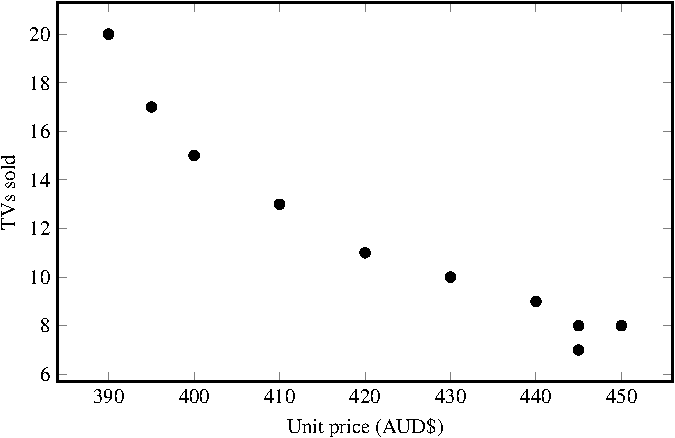
\includegraphics[scale=1.1]{image/07/fantastic-tv-scatterplot.pdf}
\caption{%%
  The price~(in Australian dollars) of each unit of FantasticTV versus
  how many units were sold across ten different stores.  The data are
  from \Table{tab:tv_sold}.
}
\label{fig:tv_sold}
\end{figure}


%%%%%%%%%%%%%%%%%%%%%%%%%%%%%%%%%%%%%%%%%%%%%%%%%%%%%%%%%%%%%%%%%%%%%%%%%%%

\subsection*{Regression formulae}

This is a job for linear regression.  Linear regression is a way to
calculate the linear function that best fits a given data set.  As you
know, a linear function has the form
\[
y
=
f(x)
=
ax + b.
\]
In the example on FantasticTV, the variable $x$ represents the price
of each unit of FantasticTV and $y = f(x)$ represents how many units
of FantasticTV were sold at $x$ dollars.

Let's see how linear regression can help you to model the data set in
\Table{tab:tv_sold}.  Denote by $x_i$ the price of each unit of
FantasticTV at store $i$.  If $i = 1$, then $x_1 = 400$ because each
unit of FantasticTV was sold for $\$400$ at store $i = 1$.  If
$i = 2$, then $x_2 = 445$.  And so on.  Then $\xbar$ denotes the
mean~(or average) price of each unit of FantasticTV across the ten
stores.  Similarly, let $y_i$ be the number of units of FantasticTV
sold at store $i$.  For $i = 1$, \Table{tab:tv_sold} shows that $y_1 =
15$ units of FantasticTV were sold at store $i = 1$.  If $i = 2$, then
$y_2 = 8$ units of FantasticTV were sold at store $i = 2$.  And so
on.  You can denote by $\ybar$ the mean~(or average) number of units
of FantasticTV sold across the ten stores.  The problem is to
approximate as best as possible the values of $a$ and $b$ in the
function $y = f(x)$.  Suppose the values of $a$ and $b$ are
approximated by $\alphahat$ and $\betahat$, respectively.  Then it can
be shown that you have the values
%%
\begin{equation}
\label{eqn:linear_regression_alpha_hat_beta_hat}
\begin{aligned}
\alphahat
&=
\frac{
  \sum_{i=1}^n (x_i - \xbar) (y_i - \ybar)
}{
  \sum_{i=1}^n (x_i - \xbar)^2
} \\[4pt]
%%
%%
\betahat
&=
\ybar - \alphahat \xbar
\end{aligned}
\end{equation}
%%
where $n$ represents the number of stores.  In particular, you have
$n = 10$ because \Table{tab:tv_sold} shows ten stores.  Sometimes it
is convenient to make the substitutions $d(x_i) = x_i - \xbar$ and
$d(y_i) = y_i - \ybar$.  You do not need to worry about how the
formulae for $\alphahat$ and $\betahat$ were derived. You need only to
worry about how to use the formulae
in~\eqref{eqn:linear_regression_alpha_hat_beta_hat}.  The data in
\Table{tab:tv_sold} can now be modelled as the linear function
\[
y
=
f(x)
=
\alphahat x + \betahat
\]
where $\alphahat$ is the rate of change of the function $y = f(x)$ and
$\betahat$ is the $y$-intercept.


%%%%%%%%%%%%%%%%%%%%%%%%%%%%%%%%%%%%%%%%%%%%%%%%%%%%%%%%%%%%%%%%%%%%%%%%%%%

\subsection*{Model the data set}

The next step is to use the formulae
in~\eqref{eqn:linear_regression_alpha_hat_beta_hat} to calculate the
rate of change and vertical intercept for the data in
\Table{tab:tv_sold}.  In general, it is very boring to calculate the
values of $\alphahat$ and $\betahat$ by hand.  You should invest some
time into learning how to use a spreadsheet software package.

Here are the major steps to perform the computation as shown
in~\eqref{eqn:linear_regression_alpha_hat_beta_hat}.  First, calculate
the values of $\xbar$ and $\ybar$.  From \Table{tab:tv_sold}, you have
\[
\xbar
=
422.5
%%
\qquad
\text{and}
\qquad
%%
\ybar
=
11.8.
\]
Next, calculate the value of $\alphahat$.  The expression
$d(x_i) = x_i - \xbar$ tells you to subtract the mean value $\xbar$
from the price of each unit of FantasticTV at store $i$.  Similarly,
the expression $d(y_i) = y_i - \ybar$ states that you subtract the
mean value $\ybar$ from the number of units sold at store $i$.
Calculate the values of $d(x_i)$ and $d(y_i)$ for each of the ten
stores.  Then for store $i$ you calculate the products
$d(x_i) \times d(y_i)$ and $d(x_i) \times d(x_i)$.  The results should
be something similar to
\Table{tab:fantastic_tv_details_regression_line}.  In
\Table{tab:fantastic_tv_details_regression_line}, sum the numbers
along the column labelled $d(x_i) d(y_i)$ to get
\[
\sum_{i=1}^n d(x_i) d(y_i)
=
-855
\]
and sum the numbers along the column labelled $d(x_i) d(x_i)$ to get
\[
\sum_{i=1}^n d(x_i) \times d(x_i)
=
4612.5.
\]
The value of $\alphahat$ can be approximated as
%%
\begin{align*}
\alphahat
&=
\frac{-855}{4612.5} \\[4pt]
&\approx
-0.185366
\end{align*}
%%
rounded to six decimal places.  The final step is to calculate the
value of $\betahat$, which can be approximated as
%%
\begin{align*}
\betahat
&=
11.8 - (\alphahat \times 422.5) \\[4pt]
&\approx
90.117073
\end{align*}
%%
rounded to six decimal places.  Therefore the number of units of
FantasticTV sold can be modelled as the linear function
\[
f(x)
=
-0.185366 x + 90.117073
\]
where $x$ represents the price of each unit of FantasticTV and $f(x)$
represents how many units of FantasticTV were sold at $x$ dollars.
\Figure{fig:fantastic_tv_regression} shows a graph of the function
$f(x)$ together with a scatter plot of the data in
\Table{tab:tv_sold}.  Note that the function $f(x)$ is a model of the
data in \Table{tab:tv_sold}.  This means that the function
approximates the data and the function gives you approximate values
for each value of $x$.  For example, for $x = 400$ you have the
approximate value of $f(400) \approx 15.97$, which is close to the
actual value of $15$.  For $x = 445$ you have $f(445) \approx 7.63$,
which is also close the actual value of $8$.

\begin{table}[!htbp]
\centering
\begin{tabular}{rrrrrr} \toprule
Price $x$ & Sold $y$ & $x_i - \xbar$ & $y_i - \ybar$ & $d(x_i)d(y_i)$ & $d(x_i)d(x_i)$ \\\midrule
$400$     & $15$     & $-22.5$       & $3.2$         & $-72$         & $506.25$       \\[4pt]
$445$     & $8$      & $22.5$        & $-3.8$        & $-85.5$       & $506.25$       \\[4pt]
$440$     & $9$      & $17.5$        & $-2.8$        & $-49$         & $306.25$       \\[4pt]
$410$     & $13$     & $-12.5$       & $1.2$         & $-15$         & $156.25$       \\[4pt]
$420$     & $11$     & $-2.5$        & $-0.8$        & $2$           & $6.25$         \\[4pt]
$430$     & $10$     & $7.5$         & $-1.8$        & $-13.5$       & $56.25$        \\[4pt]
$450$     & $8$      & $27.5$        & $-3.8$        & $-104.5$      & $756.25$       \\[4pt]
$445$     & $7$      & $22.5$        & $-4.8$        & $-108$        & $506.25$       \\[4pt]
$390$     & $20$     & $-32.5$       & $8.2$         & $-266.5$      & $1056.25$      \\[4pt]
$395$     & $17$     & $-27.5$       & $5.2$         & $-143$        & $756.25$       \\\bottomrule
\end{tabular}

\caption{%%
  Details of how to use the formulae
  in~\eqref{eqn:linear_regression_alpha_hat_beta_hat} to calculate the
  regression line for the data in \Table{tab:tv_sold}.  In most cases,
  you would need to round a number to two, four, or six decimal places
  in order to fit a table.  However, you should not round a number
  when you are calculating the values for $\alphahat$ and $\betahat$.
  The rounding should only be done after you have calculated the
  values for $\alphahat$ and $\betahat$.
}
\label{tab:fantastic_tv_details_regression_line}
\end{table}

\begin{figure}[!htbp]
\centering
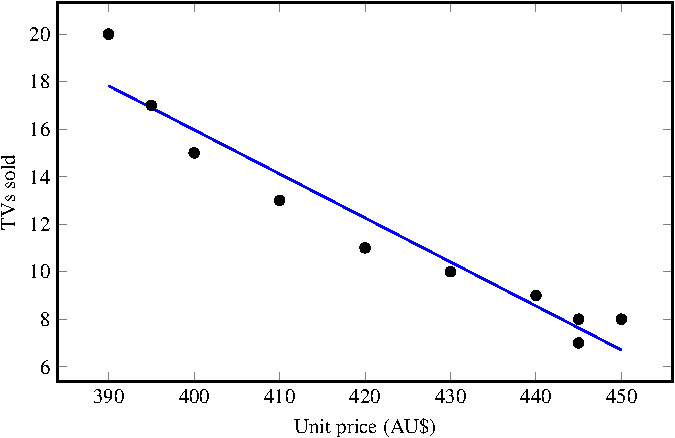
\includegraphics[scale=1]{image/07/fantastic-tv-regression.pdf}
\caption{%%
  Model the data in \Table{tab:tv_sold} with a regression line.
}
\label{fig:fantastic_tv_regression}
\end{figure}

\begin{table}[!htbp]
\centering
\begin{tabular}{cc}     \toprule
Age  & Blood pressure \\\midrule
$39$ & $144$          \\[4pt]
$47$ & $220$          \\[4pt]
$45$ & $138$          \\[4pt]
$47$ & $145$          \\[4pt]
$65$ & $162$          \\[4pt]
$46$ & $142$          \\[4pt]
$67$ & $170$          \\[4pt]
$42$ & $124$          \\[4pt]
$67$ & $158$          \\[4pt]
$56$ & $154$          \\[4pt]
$64$ & $162$          \\[4pt]
$56$ & $150$          \\[4pt]
$59$ & $140$          \\[4pt]
$34$ & $110$          \\[4pt]
$42$ & $128$          \\[4pt]
$48$ & $130$          \\[4pt]
$45$ & $135$          \\[4pt]
$17$ & $114$          \\[4pt]
$20$ & $116$          \\[4pt]
$19$ & $124$          \\[4pt]
$36$ & $136$          \\[4pt]
$50$ & $142$          \\[4pt]
$39$ & $120$          \\[4pt]
$21$ & $120$          \\[4pt]
$44$ & $160$          \\[4pt]
$53$ & $158$          \\[4pt]
$63$ & $144$          \\[4pt]
$29$ & $130$          \\[4pt]
$25$ & $125$          \\[4pt]
$69$ & $175$          \\\bottomrule
\end{tabular}

\caption{%%
  The age~(in years) and systolic blood pressure of $30$ people.
}
\label{tab:blood_pressure}
\end{table}

\begin{example}
\Table{tab:blood_pressure} shows the age and systolic blood pressure
of $30$ people.
%%
\begin{packedenum}
\item\label{subex:blood_pressure_mean_age_pressure}
  Calculate the mean age and mean blood pressure.

\item\label{subex:blood_pressure_linear_regression}
  Use linear regression to model the data in
  \Table{tab:blood_pressure}.  If a person is $70$ years old, what is
  the person's systolic blood pressure as predicted by the linear
  regression model?

\item\label{subex:blood_pressure_nonsense}
  Suppose you model the data in \Table{tab:blood_pressure} as the
  linear function $f(x) = ax + b$, where $x$ represents the age~(in
  years) of a person and $f(x)$ represents the person's systolic blood
  pressure.  Set $x = -3$ and calculate the value of $f(-3)$.  What
  does the value $f(-3)$ mean?  Explain why this value does not make
  sense.
\end{packedenum}
\end{example}

\begin{solution}
\solutionpart{subex:blood_pressure_mean_age_pressure}
Let $x$ be the age of a person and let $y$ be the person's systolic
blood pressure.  Then the mean~(or average) age is
\[
\xbar
=
\frac{1354}{30}
\approx
45
\]
years old and the mean blood pressure is
\[
\ybar
=
\frac{4276}{30}
\approx
142.53
\]
rounded to two decimal places.

\solutionpart{subex:blood_pressure_linear_regression}
You want to model the data in \Table{tab:blood_pressure} by a linear
function of the form $f(x) = ax + b$, where $x$ represents the age of
a person and $y = f(x)$ represents the person's systolic blood
pressure.  From the formulae
in~\eqref{eqn:linear_regression_alpha_hat_beta_hat} you can
approximate the values of $a$ and $b$ by $\alphahat$ and $\betahat$,
respectively.  \Table{tab:blood_pressure_regression} shows the
detailed calculation of the regression line.  Now you can approximate
$\alphahat$ as
\[
\alphahat
\approx
\frac{6585.866667}{6783.466667}
\approx
0.970870
\]
and $\betahat$ can be approximated as
\[
\betahat
=
\ybar - \alphahat \xbar
\approx
98.714718
\]
both rounded to six decimal places.  You should use a spreadsheet
software package to calculate the values of $\alphahat$ and
$\betahat$.  You should not round any number that you get during the
calculation.  Only the final results should be rounded.  The data in
\Table{tab:blood_pressure} can be modelled as the linear function
%%
\begin{equation}
\label{eqn:systolic_blood_pressure_regression}
f(x)
=
0.970870 x + 98.714718
\end{equation}
%%
where $x$ represents a person's age~(in years) and $f(x)$ represents
the person's systolic blood pressure.
\Figure{fig:blood_pressure_regression} shows a scatter plot of the
data in \Table{tab:blood_pressure} together with a graph of the
regression model~\eqref{eqn:systolic_blood_pressure_regression}.

If a person is $x = 70$ years old, the regression
model~\eqref{eqn:systolic_blood_pressure_regression} predicts that the
person would have a systolic blood pressure of
%%
\begin{align*}
f(70)
&=
(0.970870 \times 70) + 98.714718 \\[4pt]
&\approx
167
\end{align*}
%%
rounded to zero decimal places.

\begin{table}[!htbp]
\centering
\begin{tabular}{rrrrrr}                                                                      \toprule
Age $x$ & B. Pressure $y$ & $x_i - \xbar$ & $y_i - \ybar$ & $d(x_i)d(y_i)$ & $d(x_i)d(x_i)$ \\\midrule
$39$    & $144$           & $-6.133333$   & $1.466667$    & $-8.995556$   & $37.617778$    \\[4pt]
$47$    & $220$           & $1.866667$    & $77.466667$   & $144.604444$  & $3.484444$     \\[4pt]
$45$    & $138$           & $-0.133333$   & $-4.533333$   & $0.604444$    & $0.017778$     \\[4pt]
$47$    & $145$           & $1.866667$    & $2.466667$    & $4.604444$    & $3.484444$     \\[4pt]
$65$    & $162$           & $19.866667$   & $19.466667$   & $386.737778$  & $394.684444$   \\[4pt]
$46$    & $142$           & $0.866667$    & $-0.533333$   & $-0.462222$   & $0.751111$     \\[4pt]
$67$    & $170$           & $21.866667$   & $27.466667$   & $600.604444$  & $478.151111$   \\[4pt]
$42$    & $124$           & $-3.133333$   & $-18.533333$  & $58.071111$   & $9.817778$     \\[4pt]
$67$    & $158$           & $21.866667$   & $15.466667$   & $338.204444$  & $478.151111$   \\[4pt]
$56$    & $154$           & $10.866667$   & $11.466667$   & $124.604444$  & $118.084444$   \\[4pt]
$64$    & $162$           & $18.866667$   & $19.466667$   & $367.271111$  & $355.951111$   \\[4pt]
$56$    & $150$           & $10.866667$   & $7.466667$    & $81.137778$   & $118.084444$   \\[4pt]
$59$    & $140$           & $13.866667$   & $-2.533333$   & $-35.128889$  & $192.284444$   \\[4pt]
$34$    & $110$           & $-11.133333$  & $-32.533333$  & $362.204444$  & $123.951111$   \\[4pt]
$42$    & $128$           & $-3.133333$   & $-14.533333$  & $45.537778$   & $9.817778$     \\[4pt]
$48$    & $130$           & $2.866667$    & $-12.533333$  & $-35.928889$  & $8.217778$     \\[4pt]
$45$    & $135$           & $-0.133333$   & $-7.533333$   & $1.004444$    & $0.017778$     \\[4pt]
$17$    & $114$           & $-28.133333$  & $-28.533333$  & $802.737778$  & $791.484444$   \\[4pt]
$20$    & $116$           & $-25.133333$  & $-26.533333$  & $666.871111$  & $631.684444$   \\[4pt]
$19$    & $124$           & $-26.133333$  & $-18.533333$  & $484.337778$  & $682.951111$   \\[4pt]
$36$    & $136$           & $-9.133333$   & $-6.533333$   & $59.671111$   & $83.417778$    \\[4pt]
$50$    & $142$           & $4.866667$    & $-0.533333$   & $-2.595556$   & $23.684444$    \\[4pt]
$39$    & $120$           & $-6.133333$   & $-22.533333$  & $138.204444$  & $37.617778$    \\[4pt]
$21$    & $120$           & $-24.133333$  & $-22.533333$  & $543.804444$  & $582.417778$   \\[4pt]
$44$    & $160$           & $-1.133333$   & $17.466667$   & $-19.795556$  & $1.284444$     \\[4pt]
$53$    & $158$           & $7.866667$    & $15.466667$   & $121.671111$  & $61.884444$    \\[4pt]
$63$    & $144$           & $17.866667$   & $1.466667$    & $26.204444$   & $319.217778$   \\[4pt]
$29$    & $130$           & $-16.133333$  & $-12.533333$  & $202.204444$  & $260.284444$   \\[4pt]
$25$    & $125$           & $-20.133333$  & $-17.533333$  & $353.004444$  & $405.351111$   \\[4pt]
$69$    & $175$           & $23.866667$   & $32.466667$   & $774.871111$  & $569.617778$   \\\bottomrule
\end{tabular}

\caption{%%
  Detailed calculation of the regression line for the data in
  \Table{tab:blood_pressure}.  Most numbers have been rounded to six
  decimal places so as to fit the table.  However, you should not
  round numbers during the calculation.  For a big data set like
  \Table{tab:blood_pressure}, you should use a spreadsheet software
  package to calculate each number.
}
\label{tab:blood_pressure_regression}
\end{table}

\begin{figure}[!htbp]
\centering
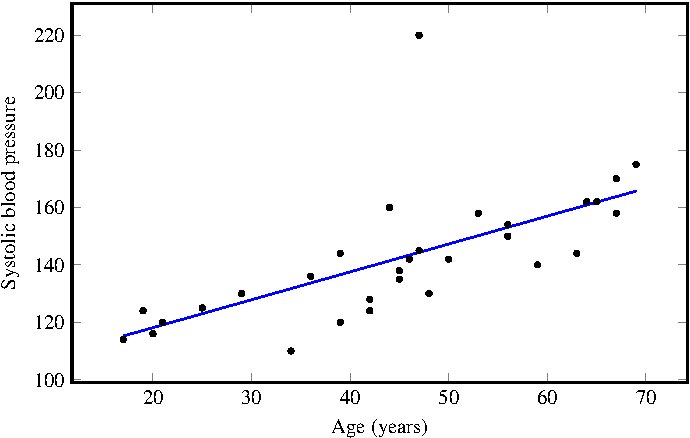
\includegraphics[scale=1]{image/07/blood-pressure-regression.pdf}
\caption{%%
  A linear regression of the data in \Table{tab:blood_pressure}.
}
\label{fig:blood_pressure_regression}
\end{figure}

\solutionpart{subex:blood_pressure_nonsense}
If a person is $x = -3$ years old, the regression
model~\eqref{eqn:systolic_blood_pressure_regression} predicts that the
person would have a systolic blood pressure of
%%
\begin{align*}
f(-3)
&=
\bigparen{0.970870 \times (-3)} + 98.714718 \\[4pt]
&\approx
96
\end{align*}
%%
rounded to zero decimal places.  The value $f(-3) \approx 96$ does not
make sense because it predicts the systolic blood pressure of someone
who is years before being born.  The data in
\Table{tab:blood_pressure} cover people who are from $17$ to $69$
years old.  The best you can say is that the regression
model~\eqref{eqn:systolic_blood_pressure_regression} is valid for
people who are between $17$ and $69$ years old.  You can use the model
to predict the systolic blood pressure of someone who is a few years
outside of what the data show.  But you should not fully trust
whatever number the regression model gives you.  The model is only an
approximation of the data.
\end{solution}

\begin{exercise}
Use linear regression to model the data in \Table{tab:height_weight}.
\end{exercise}
%%
\ifbool{showSolution}{
\begin{solution}
Let $x_i$ and $y_i$ be the height and weight, respectively, of
teenager $i$.  The mean height is
\[
\xbar
=
\frac{1738}{10}
=
173.8
\]
centimetres and the mean weight is
\[
\ybar
=
594
=
59.4
\]
kilograms.  Use the formulae
in~\eqref{eqn:linear_regression_alpha_hat_beta_hat} to produce the
data in \Table{tab:height_weight_regression}.  The value of
$\alphahat$ is obtained by summing the values along the column
labelled $d(x_i) d(y_i)$ and divide the result by the sum of the
values along the column labelled $d(x_i) d(x_i)$.  What you end up
with is the approximation
\[
\alphahat
=
\frac{137.8}{153.6}
\approx
0.897135
\]
rounded to six decimal places.  The value of $\betahat$ can be
approximated as
\[
\betahat
=
59.4 - (\alphahat \times 173.8)
\approx
-96.522135
\]
rounded to six decimal places.  Therefore the data in
\Table{tab:height_weight} can be modelled as the linear function
\[
f(x)
=
0.897135 x -96.522135
\]
where $x$ represents the height~(in centimetres) of a teenager and
$f(x)$ represents the weight~(in kilograms) of the teenager.
\Figure{fig:height_weight_regression} shows a graph of the function
$f(x)$ together with a scatter plot of the data in
\Table{tab:height_weight}.

\begin{table}[!htbp]
\centering
\begin{tabular}{rrrrrr}                                                                    \toprule
Height $x$ & Weight $y$ & $x_i - \xbar$ & $y_i - \ybar$ & $d(x_i)d(y_i)$ & $d(x_i)d(x_i)$ \\\midrule
$167$      & $51$       & $-6.8$        & $-8.4$        & $57.12$       & $46.24$        \\[4pt]
$181$      & $61$       & $7.2$         & $1.6$         & $11.52$       & $51.84$        \\[4pt]
$176$      & $69$       & $2.2$         & $9.6$         & $21.12$       & $4.84$         \\[4pt]
$173$      & $64$       & $-0.8$        & $4.6$         & $-3.68$       & $0.64$         \\[4pt]
$172$      & $65$       & $-1.8$        & $5.6$         & $-10.08$      & $3.24$         \\[4pt]
$174$      & $55$       & $0.2$         & $-4.4$        & $-0.88$       & $0.04$         \\[4pt]
$177$      & $64$       & $3.2$         & $4.6$         & $14.72$       & $10.24$        \\[4pt]
$177$      & $61$       & $3.2$         & $1.6$         & $5.12$        & $10.24$        \\[4pt]
$172$      & $50$       & $-1.8$        & $-9.4$        & $16.92$       & $3.24$         \\[4pt]
$169$      & $54$       & $-4.8$        & $-5.4$        & $25.92$       & $23.04$        \\\bottomrule
\end{tabular}

\caption{%%
  Details of using the formulae
  in~\eqref{eqn:linear_regression_alpha_hat_beta_hat} to calculate the
  regression line for the data in \Table{tab:height_weight}.
}
\label{tab:height_weight_regression}
\end{table}

\begin{figure}[!htbp]
\centering
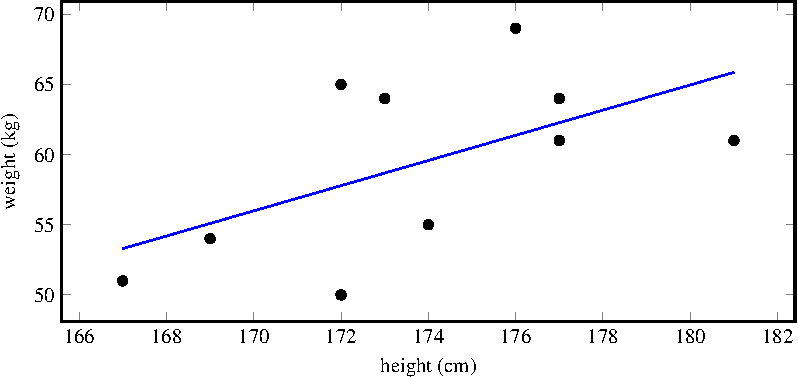
\includegraphics[scale=1]{image/07/height-weight-regression.pdf}
\caption{%%
  A regression line for the data in \Table{tab:height_weight}.
}
\label{fig:height_weight_regression}
\end{figure}
\end{solution}
}{}

\begin{exercise}
Use linear regression to model the data in \Table{tab:test_score}.
\end{exercise}
%%
\ifbool{showSolution}{
\begin{solution}
Let $x$ be the hours spent studying for a test and let $y = f(x)$ be
the corresponding test score.  From \Table{tab:test_score}, the mean
hours of studying is
\[
\xbar
=
\frac{59}{11}
\approx
5.363636
\]
and the mean test score is
\[
\ybar
=
\frac{74}{11}
\approx
6.727273
\]
both rounded to six decimal places.  Using the formulae
in~\eqref{eqn:linear_regression_alpha_hat_beta_hat} should result in
something like the values of \Table{tab:study_hours_regression}.  To
approximate the value of $\alphahat$, sum the values along the column
labelled $d(x_i) d(y_i)$, do the same for the column labelled
$d(x_i) d(x_i)$, and divide the first sum by the second sum to get the
approximation
\[
\alphahat
\approx
\frac{74.090909}{84.545455}
\approx
0.876344
\]
rounded to six decimal places.  Note that you should only do the
rounding for the final result.  The value of $\betahat$ can be
approximated as
\[
\betahat
=
\ybar - \alphahat\xbar
\approx
2.026882
\]
rounded to six decimal places.  Therefore the data in
\Table{tab:height_weight} can be modelled as the linear function
\[
f(x)
=
0.876344 x + 2.026882
\]
where $x$ represents the number of hours that a student spent studying
for a test and $f(x)$ represents the student's test score.
\Figure{fig:test_score_regression} shows a graph of the scatter plot
of the data in \Table{tab:test_score} together with the graph of the
regression function $f(x)$.

\begin{table}[!htbp]
\centering
\begin{tabular}{rrrrrr}                                                                  \toprule
Hours $x$ & Score $y$ & $x_i - \xbar$ & $y_i - \ybar$ & $d(x_i)d(y_i)$ & $d(x_i)d(x_i)$ \\\midrule
$4$       & $5$       & $-1.363636$   & $-1.727273$   & $2.355372$    & $1.859504$     \\
$3$       & $5$       & $-2.363636$   & $-1.727273$   & $4.082645$    & $5.586777$     \\
$6$       & $7$       & $0.636364$    & $0.272727$    & $0.173554$    & $0.404959$     \\
$2$       & $4$       & $-3.363636$   & $-2.727273$   & $9.173554$    & $11.314050$    \\
$1$       & $2$       & $-4.363636$   & $-4.727273$   & $20.628099$   & $19.041322$    \\
$5$       & $7$       & $-0.363636$   & $0.272727$    & $-0.099174$   & $0.132231$     \\
$8$       & $9$       & $2.636364$    & $2.272727$    & $5.991736$    & $6.950413$     \\
$9$       & $10$      & $3.636364$    & $3.272727$    & $11.900826$   & $13.223140$    \\
$4$       & $6$       & $-1.363636$   & $-0.727273$   & $0.991736$    & $1.859504$     \\
$10$      & $10$      & $4.636364$    & $3.272727$    & $15.173554$   & $21.495868$    \\
$7$       & $9$       & $1.636364$    & $2.272727$    & $3.719008$    & $2.677686$     \\\bottomrule
\end{tabular}

\caption{%%
  Detailed calculation of the regression line for the data in
  \Table{tab:test_score}.  Most values have been rounded to six
  decimal places so that the values can fit within the table.  The
  values were calculated by a spreadsheet software package.  In
  general, you should not round the values in the table.
}
\label{tab:study_hours_regression}
\end{table}

\begin{figure}[!htbp]
\centering
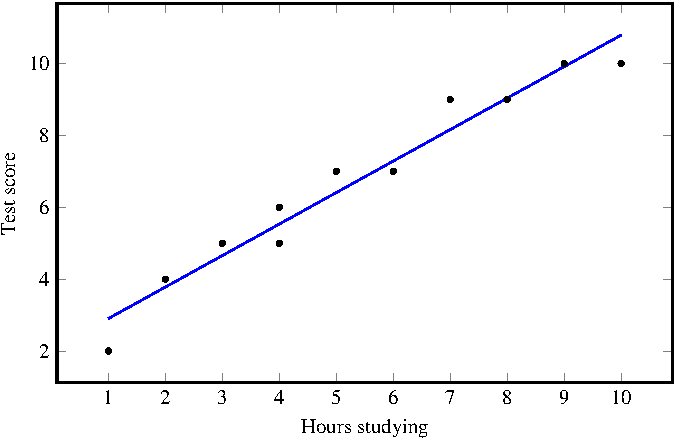
\includegraphics[scale=1]{image/07/test-score-regression.pdf}
\caption{%%
  A regression line through the data in \Table{tab:test_score}.
}
\label{fig:test_score_regression}
\end{figure}
\end{solution}
}{}


%%%%%%%%%%%%%%%%%%%%%%%%%%%%%%%%%%%%%%%%%%%%%%%%%%%%%%%%%%%%%%%%%%%%%%%%%%%

\section{Correlation coefficient}

The \emph{Pearson correlation coefficient} is a way to measure how
well a straight line fits a data set.  You know that linear regression
allows you to draw a straight line that best fits a data set.  The
straight line, or regression, function $f(x) = \alphahat x + \betahat$
is a way to approximate many pairs of numbers by a linear function.
Although the function $f(x)$ might be the best linear function to
approximate a data set, you might still ask yourself: How well does
the function $f(x)$ fit the data?  The Pearson correlation coefficient
is way to answer this question.

The Pearson correlation coefficient is usually denoted by $r$ and
defined as the number
%%
\begin{equation}
\label{eqn:Pearson_correlation_coefficient}
r
=
\frac{
  \sum_{i=1}^n (x_i - \xbar) (y_i - \ybar)
}{
  \sqrt{
    \sum_{i=1}^n (x_i - \xbar)^2 \sum_{i=1}^n (y_i - \ybar)^2
  }
}
\end{equation}
%%
where $n$ is the number of observations in the data set.  If the data
set is organised as a table, the number $n$ is also the number of rows
in the table.  You already know how to calculate the sums
\[
\sum_{i=1}^n (x_i - \xbar) (y_i - \ybar)
%%
\qquad
\text{and}
\qquad
%%
\sum_{i=1}^n (x_i - \xbar)^2.
\]
Now you need to calculate a third sum:
\[
\sum_{i=1}^n (y_i - \ybar)^2.
\]
Multiply the third sum $\sum_{i=1}^n (y_i - \ybar)^2$ by
$\sum_{i=1}^n (x_i - \xbar)^2$ and take the square root of the
resulting product.  You then divide the sum
$\sum_{i=1}^n (x_i - \xbar) (y_i - \ybar)$ by the square root to get
the number $r$.

How would you interpret the Pearson correlation coefficient as defined
by \Expression{eqn:Pearson_correlation_coefficient}?  The Pearson
correlation coefficient is a number between $-1$ and $1$, inclusive.
That is, you have $-1 \leq r \leq 1$.  Suppose you have a data set and
you have computed a regression function
$f(x) = \alphahat x + \betahat$ that best fits the data.  There are
three extreme cases to consider:
%%
\begin{packedenumeral}
\item If $r = -1$, then the function $f(x)$ fits the data perfectly.
  Every point of the data set lies on a straight line.  Furthermore,
  the rate of change of $f(x)$ is negative, i.e.~$\alphahat < 0$.

\item If $r = 1$, the function $f(x)$ fits the data perfectly.  Each
  point of the data set lies on a straight line.  The rate of change
  of $f(x)$ is positive, i.e.~$\alphahat > 0$.

\item If $r = 0$, then there is no linear relationship in the data
  set.  This does not mean that there is no relationship at all among
  the data.  The scatter plot of the data might look like a circle or
  a square or some other shape.  However, the value $r = 0$ means that
  the relationship that exists in the data, whatever that is, cannot
  be modelled as a linear function.
\end{packedenumeral}
%%
You also have values of $r \neq 0$ that are strictly between $-1$ and
$1$, i.e.~$-1 < r < 1$ and $r \neq 0$.  The following are some rough
guidelines on how to interpret the value of $r$ for a given data set:
%%
\begin{packedenumeral}
\item If $r \geq 0.9$ or $r \leq -0.9$, there is strong linear
  correlation in the data.

\item If $0.75 \leq r < 0.9$ or $-0.9 < r \leq -0.75$, there is
  moderate linear correlation in the data.

\item If $0.5 \leq r < 0.75$ or $-0.75 < r \leq -0.5$, there is weak
  linear correlation in the data.

\item If $r < 0.5$ or $r > -0.5$, there is very weak or poor linear
  correlation in the data.
\end{packedenumeral}

Here are some words of warning.  The Pearson correlation coefficient
$r$ as defined by~\eqref{eqn:Pearson_correlation_coefficient} measures
only how well a linear function fits a given data set.  The
coefficient $r$ says nothing about whether one value of the data
causes another value.  The word ``correlation'' is used in cases where
one thing~(e.g.~$B$) is observed to follow something else~(e.g.~$A$).
That is, whenever you observe $A$ you notice that you also see $B$.
The best you can say is that both of $A$ and $B$ are observed
together, they are correlated.  This does not mean that $A$ causes
$B$.  For example, suppose that whenever you go outside for a picnic
the weather starts to change and rain falls down.  You repeat this
five, ten, or fifteen times and you still see rain.  This does not
mean that you cause the rain.  You should have checked the weather
forecast and choose a nice summer day.  Correlation does not imply
causation.

\begin{table}[!htbp]
\centering
\begin{tabular}{rrrrrrr}                                                               \toprule
Height $x$ & Weight $y$ & $d(x_i)$ & $d(y_i)$ & $d(x_i)d(y_i)$ & $d(x_i)d(x_i)$ & $d(y_i)d(y_i)$ \\\midrule
$167$      & $51$       & $-6.80$  & $-8.4$   & $57.12$        & $46.24$        & $70.56$        \\[4pt]
$181$      & $61$       & $7.20$   & $1.6$    & $11.52$        & $51.84$        & $2.56$         \\[4pt]
$176$      & $69$       & $2.20$   & $9.6$    & $21.12$        & $4.84$         & $92.16$        \\[4pt]
$173$      & $64$       & $-0.80$  & $4.6$    & $-3.68$        & $0.64$         & $21.16$        \\[4pt]
$172$      & $65$       & $-1.80$  & $5.6$    & $-10.08$       & $3.24$         & $31.36$        \\[4pt]
$174$      & $55$       & $0.20$   & $-4.4$   & $-0.88$        & $0.04$         & $19.36$        \\[4pt]
$177$      & $64$       & $3.20$   & $4.6$    & $14.72$        & $10.24$        & $21.16$        \\[4pt]
$177$      & $61$       & $3.20$   & $1.6$    & $5.12$         & $10.24$        & $2.56$         \\[4pt]
$172$      & $50$       & $-1.80$  & $-9.4$   & $16.92$        & $3.24$         & $88.36$        \\[4pt]
$169$      & $54$       & $-4.80$  & $-5.4$   & $25.92$        & $23.04$        & $29.16$        \\\bottomrule
\end{tabular}

\caption{%%
  Detailed calculation of the Pearson correlation coefficient for the
  data in \Table{tab:height_weight}.  All numbers have been rounded to
  at most two decimal places in order to fit the table.  However, you
  should avoid rounding intermediate results.  Only the final numbers
  should be rounded.
}
\label{tab:height_weight_Pearson_r}
\end{table}

\begin{example}
Calculate the Pearson correlation coefficient $r$ for the data in
\Table{tab:height_weight}.  Interpret what the value of $r$ tells you
about the data in \Table{tab:height_weight}.
\end{example}

\begin{solution}
First, you use \Expression{eqn:Pearson_correlation_coefficient} to
calculate the Pearson correlation coefficient $r$.  The mean height is
approximately $\xbar \approx 173.8$ and the mean weight is
approximately $\ybar \approx 59.4$.  You use these mean values and
\Expression{eqn:Pearson_correlation_coefficient} to calculate the
value of $r$ as shown in \Table{tab:height_weight_Pearson_r}.  From
the values in \Table{tab:height_weight_Pearson_r}, you can calculate
the sum
\[
\sum_{i=1}^n (x_i - \xbar) (y_i - \ybar)
\approx
137.8
\]
and the sums
\[
\sum_{i=1}^n (x_i - \xbar)^2
\approx
153.6
%%
\qquad
\text{and}
\qquad
%%
\sum_{i=1}^n (y_i - \ybar)^2
\approx
378.4.
\]
Then the value of $r$ is approximately
%%
\begin{align*}
r
&\approx
\frac{137.8}{\sqrt{153.6 \times 378.4}} \\[4pt]
&\approx
0.57
\end{align*}
%%
rounded to two decimal places.  The value of $r \approx 0.57$ has the
following meaning.  There is a positive linear correlation between
height and weight, i.e.~taller teenagers tend to weigh heavier.
Although there is a linear relationship between the heights and
weights shown in \Table{tab:height_weight}, this linear relationship
can be described as weak.  In other words, it does not appear to be
convincing that the taller is a teenager the heavier the teenager
weighs.
\end{solution}

\begin{exercise}
Calculate the Pearson correlation coefficient $r$ for the data in
\Table{tab:test_score}.  Provide an interpretation of the value of
$r$.
\end{exercise}

\ifbool{showSolution}{
\begin{solution}
First, you use \Expression{eqn:Pearson_correlation_coefficient} to
calculate the Pearson correlation coefficient $r$.  The mean hours of
study is $\xbar \approx 5.36$ and the mean test score is
$\ybar \approx 6.73$, both rounded to two decimal places.  Use these
mean values and \Expression{eqn:Pearson_correlation_coefficient} to
calculate the values shown in \Table{tab:test_score_pearson}.  Use the
values in \Table{tab:test_score_pearson} to calculate the sum
\[
\sum_{i=1}^n (x_i - \xbar) (y_i - \ybar)
\approx
74.09
\]
and the sums
\[
\sum_{i=1}^n (x_i - \xbar)^2
\approx
84.55
%%
\qquad
\text{and}
\qquad
%%
\sum_{i=1}^n (y_i - \ybar)^2
\approx
68.18
\]
all rounded to two decimal places.  Then the value of $r$ is
approximately
%%
\begin{align*}
r
&\approx
\frac{
  74.09
}{
  \sqrt{84.55 \times 68.18}
} \\[4pt]
&\approx
0.9759
\end{align*}
%%
rounded to four decimal places.

\begin{table}[!htbp]
\centering
\begin{tabular}{rrrrrrr}                                                                        \toprule
Hours $x$ & Score $y$ & $d(x_i)$ & $d(y_i)$ & $d(x_i)d(y_i)$ & $d(x_i)d(x_i)$ & $d(y_i)d(y_i)$ \\\midrule
$4$       & $5$       & $-1.36$  & $-1.73$  & $2.36$        & $1.86$         & $2.98$         \\
$3$       & $5$       & $-2.36$  & $-1.73$  & $4.08$        & $5.59$         & $2.98$         \\
$6$       & $7$       & $0.64$   & $0.27$   & $0.17$        & $0.40$         & $0.07$         \\
$2$       & $4$       & $-3.36$  & $-2.73$  & $9.17$        & $11.31$        & $7.44$         \\
$1$       & $2$       & $-4.36$  & $-4.73$  & $20.63$       & $19.04$        & $22.35$        \\
$5$       & $7$       & $-0.36$  & $0.27$   & $-0.10$       & $0.13$         & $0.07$         \\
$8$       & $9$       & $2.64$   & $2.27$   & $5.99$        & $6.95$         & $5.17$         \\
$9$       & $10$      & $3.64$   & $3.27$   & $11.90$       & $13.22$        & $10.71$        \\
$4$       & $6$       & $-1.36$  & $-0.73$  & $0.99$        & $1.86$         & $0.53$         \\
$10$      & $10$      & $4.64$   & $3.27$   & $15.17$       & $21.50$        & $10.71$        \\
$7$       & $9$       & $1.64$   & $2.27$   & $3.72$        & $2.68$         & $5.17$         \\\bottomrule
\end{tabular}

\caption{%%
  Detailed calculation of the Pearson correlation coefficient for the
  data in \Table{tab:test_score}.  Most values have been rounded to
  two decimal places so as to fit the table.  However, you should only
  round the final results, not the intermediate values.
}
\label{tab:test_score_pearson}
\end{table}

The value of $r \geq 0.9$ suggests a strong linear correlation between
the hours spent studying for a test and the test scores.  In
particular, the correlation is positive, meaning that the more hours
that a student spent on studying for a test the higher is the
student's test score.  Note that correlation is not the same as
causation.  The data in \Table{tab:test_score} suggests a strong
positive linear correlation between hours spent studying for a test
and the test scores.  You should not interpret the high value of $r$
as saying that more hours spent studying for a test causes higher test
scores.  Other factors not given by the data might have contributed to
a student's test score.  For example, the students with high or
perfect test scores might have been studying every day since the start
of the school year.
\end{solution}
}{}


\newpage
%%%%%%%%%%%%%%%%%%%%%%%%%%%%%%%%%%%%%%%%%%%%%%%%%%%%%%%%%%%%%%%%%%%%%%%%%%%

\section*{Problem}

\begin{problem}
\item Read the following article by Brian Hayes:
  \emph{Gauss' day of reckoning}.

\item\label{prob:sum_even_number_of_terms_20}
  Consider the problem of summing the first $20$ positive integers:
  \[
  S
  =
  \sumseq{1 + 2}{3}{20}.
  \]
  What you want to do is calculate the value of the sum $S$ by means
  of a formula.  The $20$ integers can be divided into two groups.
  One group consists of the integers from $1$ to $10$, inclusive.  The
  second group consists of the integers from $11$ to $20$, inclusive.
  On one line, write the numbers from $1$ to $10$ in increasing order.
  On the next line, write the numbers from $11$ to $20$ in decreasing
  order.  What you should get is that $20$ is underneath $1$, $19$ is
  underneath $2$, $18$ is underneath $3$, and so on, up to $11$ being
  underneath $10$.  Thus you have ten columns and two rows.
  %%
  \begin{packedenum}
  \item\label{subprob:sum_even_number_add_column}
    Add the two numbers in each column and write the sum underneath
    the two numbers.  You should now have three rows, where the third
    row gives you the column sums.

  \item\label{subprob:sum_even_number_observation}
    What do you notice about the numbers in the third row?

  \item\label{subprob:sum_even_number_sum}
    Use the numbers in the third row to calculate the value of the sum
    $S$.
  \end{packedenum}
\ifbool{showSolution}{
\begin{solution}
\solutionpart{subprob:sum_even_number_add_column}
After adding the two numbers in each column, you now have the
following table:
\[
\begin{matrix}
1  & 2  & 3  & 4  & 5  & 6  & 7  & 8  & 9  & 10 \\[4pt]
20 & 19 & 18 & 17 & 16 & 15 & 14 & 13 & 12 & 11 \\\midrule
21 & 21 & 21 & 21 & 21 & 21 & 21 & 21 & 21 & 21
\end{matrix}
\]

\solutionpart{subprob:sum_even_number_observation}
The numbers in the third row are all the same.

\solutionpart{subprob:sum_even_number_sum}
In the third row, the integer $21$ occurs ten times.  The sum of the
numbers in the third row is $10 \times 21 = 210$.  Conclude that the
value of the sum $S$ is $S = 210$.
\end{solution}
}{}

\item\label{prob:sum_even_number_of_terms_formula}
  This problem will help you to derive a formula for the sum of the
  first $n \geq 1$ positive integers, where $n$ is even.
  %%
  \begin{packedenum}
  \item\label{subprob:sum_even_number_50}
    Use the technique from \Problem{prob:sum_even_number_of_terms_20}
    to calculate the sum of all integers from $1$ up to $50$,
    inclusive.

  \item\label{subprob:sum_even_number_100}
    Use the technique from \Problem{prob:sum_even_number_of_terms_20}
    to calculate the sum of all integers from $1$ up to $100$,
    inclusive.

  \item\label{subprob:sum_even_number_formula}
    Let $n \geq 1$ be an even integer.  Consider the problem of
    calculating the sum
    \[
    S
    =
    \sumseq{1 + 2}{3}{n}.
    \]
    Derive a formula to calculate the sum $S$.
  \end{packedenum}
\ifbool{showSolution}{
\begin{solution}
\solutionpart{subprob:sum_even_number_50}
The integers from $1$ to $50$ can be divided into two groups.  One
group consists of the integers from $1$ to $25$, inclusive.  The other
group consists of the integers from $26$ to $50$, inclusive.  What you
end up with is the following table:
\[
\begin{matrix}
1  & 2  & 3  & 4  & \cdots & 24 & 25 \\[4pt]
50 & 49 & 48 & 47 & \cdots & 27 & 26
\end{matrix}
\]
You have the sum $1 + 50 = 51$, which occurs as the column sum in each
of the $25$ columns.  Then you have $51 \times 25 = 1275$, which is
the sum of the integers from $1$ to $50$, inclusive.

\solutionpart{subprob:sum_even_number_100}
Divide the integers from $1$ to $100$ into two rows.  The first row
consists of the integers from $1$ to $50$, inclusive.  In the second
row, you have the integers from $51$ to $100$, inclusive.  You now
have the following table:
\[
\begin{matrix}
1   & 2  & 3  & 4  & \cdots & 49 & 50 \\[4pt]
100 & 99 & 98 & 97 & \cdots & 52 & 51
\end{matrix}
\]
You have the sum $1 + 100 = 101$, which occurs as the column sum in
each of the $50$ columns.  Then $101 \times 50 = 5050$ is the sum of
the positive integers from $1$ to $100$, inclusive.

\solutionpart{subprob:sum_even_number_formula}
Since $n$ is positive and even, you can write $n$ as the expression
$n = 2k$, where $k$ is a positive integer.  Now divide the integers
from $1$ to $n$, inclusive, into two rows.  In the first row, you have
the integers from $1$ to $k$, inclusive.  In the second row, you have
the integers from $k + 1$ to $n$, inclusive.  You have the sum
$n + 1$, which is the column sum in each of the $k$ columns.  Thus
$(n + 1) \times k$ is the sum of the positive integers from $1$ to
$n$, inclusive, where $n \geq 1$ is even.
\end{solution}
}{}

\item This problem is similar to
  \Problem{prob:sum_even_number_of_terms_formula}, but $n \geq 1$ is
  now assumed to be an odd integer.
  %%
  \begin{packedenum}
  \item\label{subprob:sum_integers_from_1_to_35}
    To sum all the positive integers from $1$ to $35$, inclusive, you
    use the technique from
    \Problem{prob:sum_even_number_of_terms_formula} to sum the
    integers from $1$ to $34$, inclusive.  Then you add $35$ to your
    result.  Use the above procedure to add up all the positive
    integers from $1$ to $35$, inclusive.

  \item\label{subprob:sum_integers_from_1_to_51}
    Use the technique from \Part{subprob:sum_integers_from_1_to_35} to
    calculate the sum of the integers from $1$ to $51$, inclusive.

  \item\label{subprob:sum_integers_n_odd}
    Let $n \geq 1$ be an odd integer and consider the sum
    \[
    S
    =
    \sumseq{1 + 2}{3}{n}.
    \]
    Prove that the sum can also be written as
    \[
    S
    =
    \frac{
      n(n + 1)
    }{
      2
    }.
    \]
  \end{packedenum}
\ifbool{showSolution}{
\begin{solution}
\solutionpart{subprob:sum_integers_from_1_to_35}
First, let's calculate the sum of the integers from $1$ to $34$,
inclusive.  On one row, you have the integers from $1$ to $17$ in
increasing order.  On the next row, you have the integers from $18$ to
$34$ in decreasing order.  You have the sum $1 + 34 = 35$, which
occurs as the column sum of each of $17$ columns.  Thus
\[
\sumseq{1 + 2}{3}{34}
=
35 \times 17
=
595.
\]
Finally, you add $35$ to your result to get
\[
(35 \times 17) + 35
=
595 + 35
=
630
\]
which is the sum of the integers from $1$ to $35$, inclusive.

\solutionpart{subprob:sum_integers_from_1_to_51}
To calculate the sum of the integers from $1$ to $51$, inclusive, you
first use the technique from
\Problem{prob:sum_even_number_of_terms_formula} to calculate the sum
from $1$ to $50$, inclusive.  Then you add $51$ to your result.  The
sum of the integers from $1$ to $50$, inclusive, is given by
\[
(1 + 50) \times 25
=
51 \times 25
=
1275
\]
because you have $25$ columns, each of which has the column sum of
$51$.  Now add $51$ to your result to get
\[
(51 \times 25) + 51
=
1326
\]
which is the sum of the integers from $1$ to $51$, inclusive.

\solutionpart{subprob:sum_integers_n_odd}
Since $n \geq 1$ is odd, it can be written as $n = 2k + 1$, where $k$
is a positive integer.  Then $n - 1 = 2k$ is even and solving the
latter expression for $k$ shows that
%%
\begin{equation}
\label{eqn:n_odd_define_k}
k
=
\frac{n - 1}{2}.
\end{equation}
%%
Use
\Subproblem{prob:sum_even_number_of_terms_formula}{subprob:sum_even_number_formula}
to calculate the sum of the integers from $1$ to $n - 1$, inclusive.
The sum is
\[
\bigparen{(n - 1) + 1}k
=
nk.
\]
Now add $n$ to the result and use the definition of $k$ as in
\Equation{eqn:n_odd_define_k} to get
%%
\begin{align*}
nk + n
&=
n(k + 1) \\[4pt]
&=
n
\parenthesis*{
  \frac{n-1}{2}
  +
  1
} \\[4pt]
&=
n
\parenthesis*{
  \frac{n-1}{2}
  +
  \frac{2}{2}
} \\[4pt]
&=
\frac{n(n + 1)}{2}
\end{align*}
%%
which is what you were required to prove.
\end{solution}
}{}

\item You will derive a formula to sum the first $n$ positive
  integers, regardless of whether $n$ is even or odd.
  %%
  \begin{packedenum}
  \item\label{subprob:sum_first_10}
    As an example, consider the problem of summing the integers from
    $1$ to $10$, inclusive.  That is, you want to calculate the sum
    \[
    S
    =
    \sumseq{1 + 2}{3}{10}.
    \]
    On one row, write the integers from $1$ to $10$ in increasing
    order.  On the next row, write the same ten integers but in
    decreasing order.  Now $10$ should be underneath $1$, $9$
    underneath $2$, and so on, down to $1$ being underneath $10$.
    Thus you have two rows and ten columns as in the following table:
    \[
    \begin{matrix}
    1  & 2 & 3 & \cdots & 10 \\[4pt]
    10 & 9 & 8 & \cdots & 1
    \end{matrix}
    \]
    Note that if you add together the numbers in the first row, you
    would get the sum $S$.  Adding the numbers in the second row would
    also give you the sum $S$.  Calculate the column sum and note that
    this number occurs as the sum in each column.  Multiplying the
    column sum by $10$~(i.e.~the number of columns) and you get twice
    the value of $S$, which is $2S$.  However, you want $S$, not $2S$
    so you divide by $2$ to get $S$.  Use the above procedure to
    determine the sum of the integers from $1$ to $10$, inclusive.

  \item\label{subprob:sum_first_100}
    Use the technique from \Part{subprob:sum_first_10} to sum the
    integers from $1$ to $100$, inclusive.

  \item\label{subprob:sum_first_n_positive}
    Let $n \geq 1$ be an integer and consider the sum
    \[
    S
    =
    \sumseq{1 + 2}{3}{n}
    \]
    of the first $n$ positive integers.  Prove that $S$ can be written
    as
    \[
    S
    =
    \frac{n(n + 1)}{2}.
    \]
  \end{packedenum}
\ifbool{showSolution}{
\begin{solution}
\solutionpart{subprob:sum_first_10}
Each column has a sum of $1 + 10 = 11$.  As there are $10$ columns,
the sum of the third row is $11 \times 10 = 110$, which is twice of
$S$.  That is, you have
\[
2S
=
110.
\]
Solving for $S$ shows that $S = 110 / 2 = 55$.  Therefore $S = 55$ is
the sum of the integers from $1$ to $10$, inclusive.

\solutionpart{subprob:sum_first_100}
Let $S$ be the sum of the integers from $1$ to $100$, inclusive.  On
the first row, you write the integers from $1$ to $100$ in increasing
order.  On the next row, you write the integers from $1$ to $100$ in
decreasing order.  What you end up with is the following table:
\[
\begin{matrix}
1   & 2  & 3  & \cdots & 100 \\[4pt]
100 & 99 & 98 & \cdots & 1
\end{matrix}
\]
Each column has a sum of $1 + 100 = 101$.  Since there are $100$
columns, the sum of the third row is $101 \times 100$, which is twice
of $S$.  That is, you have $2S = 101 \times 100$.  Solving for $S$
results in
\[
S
=
\frac{101 \times 100}{2}
=
101 \times 50
=
5050.
\]
Thus $S = 5050$ is the sum of the integers from $1$ to $100$,
inclusive.

\solutionpart{subprob:sum_first_n_positive}
You use the same technique as
in \Parts{subprob:sum_first_10}{subprob:sum_first_100}.  On one row,
you write the integers from $1$ to $n$, inclusive, in increasing
order.  On the next row, you write the integers from $1$ to $n$ in
decreasing order.  You then have the following table:
\[
\begin{matrix}
1 & 2   & 3   & \cdots & n \\[4pt]
n & n-1 & n-2 & \cdots & 1
\end{matrix}
\]
Each column has the sum $n + 1$.  Since there are $n$ columns, then
the sum of the third row is $n(n + 1)$, which is twice the value of
$S$.  That is, you have
\[
2S
=
n(n + 1).
\]
Solving the last equation for $S$ results in $S = \frac{n(n+1)}{2}$ as
required.
\end{solution}
}{}

\begin{table}[!htbp]
\centering
\begin{tabular}{cc} \toprule
Age   & Eggs      \\\midrule
$4$   & $5$       \\
$5$   & $6$       \\
$6$   & $4$       \\
$7$   & $5$       \\
$8$   & $5$       \\
$9$   & $4$       \\
$10$  & $4$       \\
$11$  & $4$       \\
$12$  & $3$       \\
$13$  & $4$       \\
$14$  & $3$       \\
$15$  & $2$       \\
$16$  & $3$       \\
$17$  & $2$       \\\bottomrule
\end{tabular}

\caption{%%
  The age of a hen versus the number of eggs that she laid per week.
  Age is measured in months.
}
\label{tab:age_egg}
\end{table}

\item \Table{tab:age_egg} shows the age of a hen and the number of
  eggs that she laid per week.
  %%
  \begin{packedenum}
  \item\label{subprob:hen_eggs_scatterplot}
    Graph the data in the table as a scatter plot.  What can you
    conclude from the scatter plot?

  \item\label{subprob:hen_eggs_regression}
    Use linear regression to model the data in \Table{tab:age_egg}.

  \item\label{subprob:hen_eggs_correlation}
    Calculate the Pearson correlation coefficient $r$ for the data in
    \Table{tab:age_egg}.  Provide an interpretation of the value of
    $r$.
  \end{packedenum}
\ifbool{showSolution}{
\begin{solution}
\solutionpart{subprob:hen_eggs_scatterplot}
\Figure{fig:age_egg} shows a scatter plot of the data in
\Table{tab:age_egg}.  Without any additional information, apart from
what is presented in the table, the graph shows that as the hen gets
older she lays fewer eggs per week.

\begin{figure}[!htbp]
\centering
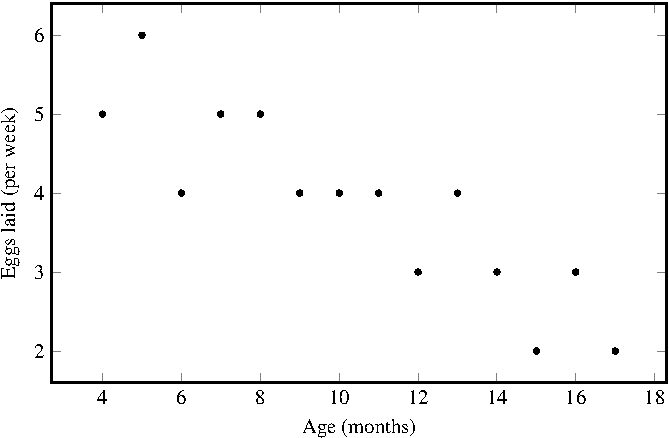
\includegraphics[scale=1]{image/07/age-eggs-scatterplot.pdf}
\caption{%%
  The number of eggs that a hen laid per week versus her age in
  months.  The data are from \Table{tab:age_egg}.
}
\label{fig:age_egg}
\end{figure}

\solutionpart{subprob:hen_eggs_regression}
Let $x$ be the age~(in months) of the hen and let $y = f(x)$ be the
number of eggs that the hen laid per week when she was at age $x$.
Using the data in \Table{tab:age_egg}, the mean age is
\[
\xbar
=
\frac{147}{14}
=
10.5
\]
months and the mean number of eggs is
\[
\ybar
=
\frac{54}{14}
\approx
3.857143
\]
per week, rounded to six decimal places.  Use the formulae
in~\eqref{eqn:linear_regression_alpha_hat_beta_hat} to obtain the
values in \Table{tab:age_egg_regression}.  To approximate the value of
$\alphahat$, sum the values along the column labelled $d(x_i) d(y_i)$,
do the same for the column labelled $d(x_i) d(x_i)$, and divide the
first sum by the second sum to obtain the approximation
\[
\alphahat
=
\frac{-56}{227.5}
\approx
-0.246154
\]
rounded to six decimal places.  The value of $\betahat$ can be
approximated as
\[
\betahat
=
\ybar - \alphahat \xbar
\approx
6.441758
\]
rounded to six decimal places.  Therefore the data in
\Table{tab:age_egg} can be modelled as the linear function
\[
f(x)
=
-0.246154 x + 6.441758
\]
where $x$ represents the age~(in months) of a hen and $f(x)$
represents the number of eggs that she lay per week at $x$ months
old.  \Figure{fig:age_eggs_regression} shows a scatter plot of the
data in \Table{tab:age_egg} together with a graph of the function
$f(x)$.

\begin{table}[!htbp]
\centering
\begin{tabular}{rrrrrr}                                                               \toprule
Age $x$ & Eggs $y$ & $x_i - \xbar$ & $y_i - \ybar$ & $d(x_i)d(y_i)$ & $d(x_i)d(x_i)$ \\\midrule
$4$     & $5$      & $-6.5$        & $1.142857$    & $-7.428571$   & $42.25$        \\
$5$     & $6$      & $-5.5$        & $2.142857$    & $-11.785714$  & $30.25$        \\
$6$     & $4$      & $-4.5$        & $0.142857$    & $-0.642857$   & $20.25$        \\
$7$     & $5$      & $-3.5$        & $1.142857$    & $-4.000000$   & $12.25$        \\
$8$     & $5$      & $-2.5$        & $1.142857$    & $-2.857143$   & $6.25$         \\
$9$     & $4$      & $-1.5$        & $0.142857$    & $-0.214286$   & $2.25$         \\
$10$    & $4$      & $-0.5$        & $0.142857$    & $-0.071429$   & $0.25$         \\
$11$    & $4$      & $0.5$         & $0.142857$    & $0.071429$    & $0.25$         \\
$12$    & $3$      & $1.5$         & $-0.857143$   & $-1.285714$   & $2.25$         \\
$13$    & $4$      & $2.5$         & $0.142857$    & $0.357143$    & $6.25$         \\
$14$    & $3$      & $3.5$         & $-0.857143$   & $-3.000000$   & $12.25$        \\
$15$    & $2$      & $4.5$         & $-1.857143$   & $-8.357143$   & $20.25$        \\
$16$    & $3$      & $5.5$         & $-0.857143$   & $-4.714286$   & $30.25$        \\
$17$    & $2$      & $6.5$         & $-1.857143$   & $-12.071429$  & $42.25$        \\\bottomrule
\end{tabular}

\caption{%%
  Detailed calculation of the regression line for the data in
  \Table{tab:age_egg}.  Note that most numbers have been rounded to
  six decimal places in order to fit the table.  You should only do
  the rounding for the final results.  Except for the first two
  columns, the numbers in the table should be computed by using a
  spreadsheet software package.
}
\label{tab:age_egg_regression}
\end{table}

\begin{figure}[!htbp]
\centering
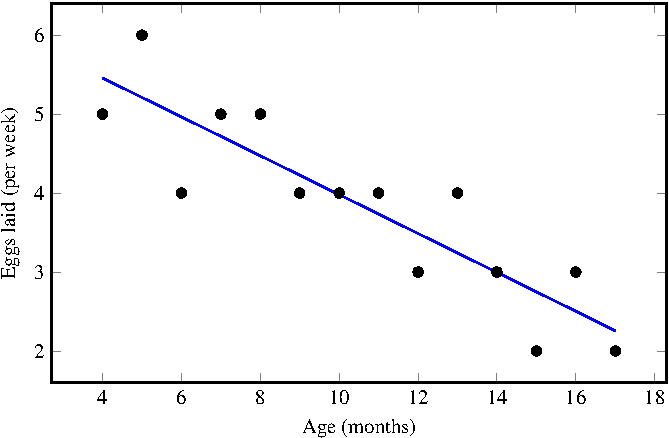
\includegraphics[scale=1]{image/07/age-eggs-regression.pdf}
\caption{%%
  A regression line through the data in \Table{tab:age_egg}.
}
\label{fig:age_eggs_regression}
\end{figure}

\solutionpart{subprob:hen_eggs_correlation}
First, you use \Expression{eqn:Pearson_correlation_coefficient} to
calculate the Pearson correlation coefficient.  The mean age is
$\xbar \approx 10.5$ months and the mean number of eggs
$\ybar \approx 3.9$, both figures rounded to one decimal place.  Use
the mean values and \Expression{eqn:Pearson_correlation_coefficient}
to calculate the values shown in \Table{tab:age_egg_pearson}.  Use the
values in \Table{tab:age_egg_pearson} to calculate the sum
\[
\sum_{i=1}^n (x_i - \xbar) (y_i - \ybar)
=
-56
\]
and the sums
\[
\sum_{i=1}^n (x_i - \xbar)^2
=
227.5
%%
\qquad
\text{and}
\qquad
%%
\sum_{i=1}^n (y_i - \ybar)^2
\approx
17.71
\]
where the last sum has been rounded to two decimal places.  The value
of $r$ is approximately
%%
\begin{align*}
r
&\approx
\frac{
  -56
}{
  \sqrt{
    227.5 \times 17.71
  }
} \\[4pt]
&\approx
-0.8821
\end{align*}
%%
rounded to four decimal places.

\begin{table}[!htbp]
\centering
\begin{tabular}{rrrrrrr}                                                              \toprule
$x$  & $y$ & $d(x_i)$ & $d(y_i)$ & $d(x_i)d(y_i)$ & $d(x_i)d(x_i)$  & $d(y_i)d(y_i)$ \\\midrule
$4$  & $5$ & $-6.5$   & $1.14$   & $-7.43$       & $42.25$         & $1.31$         \\
$5$  & $6$ & $-5.5$   & $2.14$   & $-11.79$      & $30.25$         & $4.59$         \\
$6$  & $4$ & $-4.5$   & $0.14$   & $-0.64$       & $20.25$         & $0.02$         \\
$7$  & $5$ & $-3.5$   & $1.14$   & $-4$          & $12.25$         & $1.31$         \\
$8$  & $5$ & $-2.5$   & $1.14$   & $-2.86$       & $6.25$          & $1.31$         \\
$9$  & $4$ & $-1.5$   & $0.14$   & $-0.21$       & $2.25$          & $0.02$         \\
$10$ & $4$ & $-0.5$   & $0.14$   & $-0.07$       & $0.25$          & $0.02$         \\
$11$ & $4$ & $0.5$    & $0.14$   & $0.071$       & $0.25$          & $0.02$         \\
$12$ & $3$ & $1.5$    & $-0.86$  & $-1.29$       & $2.25$          & $0.73$         \\
$13$ & $4$ & $2.5$    & $0.14$   & $0.36$        & $6.25$          & $0.02$         \\
$14$ & $3$ & $3.5$    & $-0.86$  & $-3$          & $12.25$         & $0.73$         \\
$15$ & $2$ & $4.5$    & $-1.86$  & $-8.36$       & $20.25$         & $3.45$         \\
$16$ & $3$ & $5.5$    & $-0.86$  & $-4.71$       & $30.25$         & $0.73$         \\
$17$ & $2$ & $6.5$    & $-1.86$  & $-12.07$      & $42.25$         & $3.45$         \\\bottomrule
\end{tabular}

\caption{%%
  Detailed calculation of the Pearson correlation coefficient for the
  data in \Table{tab:age_egg}.  The column for $x$ is for the age in
  months and the column for $y$ is the number of eggs per week.  Note
  that most values have been rounded to two decimal places in order to
  fit the table.  However, you should only round the final result.
}
\label{tab:age_egg_pearson}
\end{table}

The value of $-0.9 < -0.8821 \leq -0.75$ tells you that there is
moderate linear correlation in the data of \Table{tab:age_egg}.  In
particular, the correlation coefficient tells you that as the hen gets
older it tends to lay fewer eggs per week.
\end{solution}
}{}

\item This problem will help you to understand the idea of the
  \emph{convergence of an infinite sum}.  You know that you get a sum
  when you add together a bunch of numbers.  An infinite sum is
  similar.  However, the only difference is that an infinite sum has
  an infinite number of terms.  Here, you will consider the infinite
  sum
  %%
  \begin{equation}
  \label{eqn:Basel_problem}
  \sum_{k=1}^\infty \frac{1}{k^2}
  =
  \sumi{
    \frac{1}{1^2}
  }{
    \frac{1}{2^2}
  }{
    \frac{1}{3^2}
  }
  \end{equation}
  %%
  which has the property that it does not grow as large as you want as
  you add more and more terms to the sum.  This is counter-intuitive
  because you know that if you add the first ten positive integers,
  you get a sum.  If you add more and more positive integers together
  you get a larger sum.  So it is rather strange that there are cases
  where you can add together an infinite number of terms without the
  sum ever becoming as large as you want.
  %%
  \begin{packedenum}
  \item\label{subprob:Basel_problem_sum_first_5}
    Consider the first five terms in \Expression{eqn:Basel_problem}.
    The sum of these first five terms would be written as
    %%
    \begin{equation}
    \label{eqn:Basel_problem_sum_first_5}
    \sum_{k=1}^5 \frac{1}{k^2}
    =
    \frac{1}{1^2} + \frac{1}{2^2} + \frac{1}{3^2}
    +
    \frac{1}{4^2} + \frac{1}{5^2}.
    \end{equation}
    %%
    Use Excel or any other computer program to calculate the
    sum~\eqref{eqn:Basel_problem_sum_first_5}.

  \item\label{subprob:Basel_problem_sum_first_10}
    The sum of the first ten terms in \Expression{eqn:Basel_problem}
    would be written as
    %%
    \begin{equation}
    \label{eqn:Basel_problem_sum_first_10}
    \sum_{k=1}^{10} \frac{1}{k^2}
    =
    \frac{1}{1^2} + \frac{1}{2^2} + \frac{1}{3^2}
    +
    \frac{1}{4^2} + \frac{1}{5^2}
    +
    \frac{1}{6^2} + \frac{1}{7^2} + \frac{1}{8^2}
    +
    \frac{1}{9^2} + \frac{1}{10^2}.
    \end{equation}
    %%
    Calculate the sum~\eqref{eqn:Basel_problem_sum_first_10}.

  \item\label{subprob:Basel_problem_sum_first_100}
    Calculate the sum of the first $100$ terms in
    \Expression{eqn:Basel_problem}.

  \item\label{subprob:Basel_problem_sum_first_1000}
    Repeat \Part{subprob:Basel_problem_sum_first_100} for $200$ terms,
    $300$ terms, $400$ terms, $500$ terms, $600$ terms, $700$ terms,
    $800$ terms, $900$ terms, and $1000$ terms.  Organise your results
    since \Part{subprob:Basel_problem_sum_first_5} into a table that
    has two columns and $13$ rows.  The first row has the column
    headings.  Produce a scatter plot of the data in your table.

  \item\label{subprob:Basel_problem_approximate_value}
    Carefully look over your table of values and the scatter plot.
    Suppose that you sum not only $1000$ terms, but $10,000$ terms or
    $100,000$ terms or as many terms as you want.  As the number of
    terms increases, guess the value of the true sum.  The true value
    of \Expression{eqn:Basel_problem} is a fixed number and you would
    say that \Expression{eqn:Basel_problem} \emph{converges} to that
    fixed number, whatever value it happens to be.
  \end{packedenum}
\ifbool{showSolution}{
\begin{solution}
\solutionpart{subprob:Basel_problem_sum_first_5}
The sum of the first five terms in \Expression{eqn:Basel_problem} is
approximately
\[
\sum_{k=1}^5 \frac{1}{k^2}
=
\frac{1}{1^2}
+
\frac{1}{2^2}
+
\frac{1}{3^2}
+
\frac{1}{4^2}
+
\frac{1}{5^2}
\approx
1.463611
\]
rounded to six decimal places.

\solutionpart{subprob:Basel_problem_sum_first_10}
In \Expression{eqn:Basel_problem} the sum of the first ten terms is
approximately
\[
\sum_{k=1}^{10} \frac{1}{k^2}
=
\sumseq{
  \frac{1}{1^2}
  +
  \frac{1}{2^2}
}{
  \frac{1}{3^2}
}{
  \frac{1}{10^2}
}
\approx
1.549768
\]
rounded to six decimal places.

\solutionpart{subprob:Basel_problem_sum_first_100}
In \Expression{eqn:Basel_problem} the sum of the first $100$ terms is
approximately
\[
\sum_{k=1}^{100} \frac{1}{k^2}
=
\sumseq{
  \frac{1}{1^2}
  +
  \frac{1}{2^2}
}{
  \frac{1}{3^2}
}{
  \frac{1}{100^2}
}
\approx
1.634984
\]
rounded to six decimal places.

\solutionpart{subprob:Basel_problem_sum_first_1000}
\Table{tab:Basel_problem_approximate_sums} lists some approximate sums
of \Expression{eqn:Basel_problem}.  See
\Figure{fig:Basel_problem_approximate_sums} for a scatter plot of the
data in the table.

\begin{table}[!htbp]
\centering
\begin{tabular}{rl}    \toprule
Terms   & Sum        \\\midrule
$5$     & $1.463611$ \\[4pt]
$10$    & $1.549768$ \\[4pt]
$100$   & $1.634984$ \\[4pt]
$200$   & $1.639947$ \\[4pt]
$300$   & $1.641606$ \\[4pt]
$400$   & $1.642437$ \\[4pt]
$500$   & $1.642936$ \\[4pt]
$600$   & $1.643269$ \\[4pt]
$700$   & $1.643507$ \\[4pt]
$800$   & $1.643685$ \\[4pt]
$900$   & $1.643824$ \\[4pt]
$1000$  & $1.643935$ \\\bottomrule
\end{tabular}

\caption{%%
  Approximate sums of \Expression{eqn:Basel_problem}.
}
\label{tab:Basel_problem_approximate_sums}
\end{table}

\begin{figure}[!htbp]
\centering
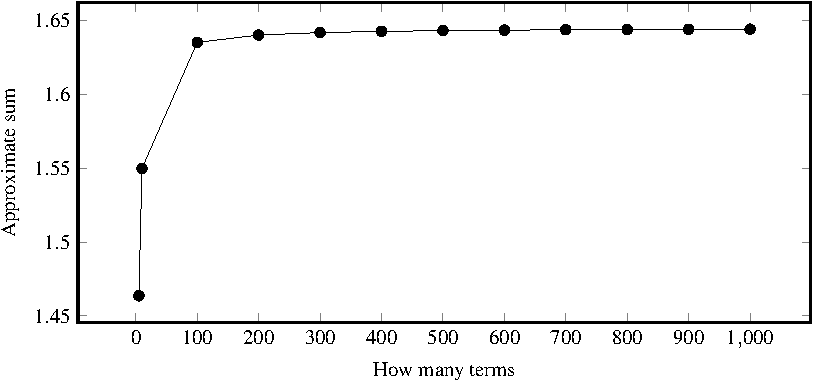
\includegraphics[scale=1]{image/07/basel-problem-scatterplot.pdf}
\caption{%%
  Scatter plot of the number of terms in
  \Expression{eqn:Basel_problem} versus the corresponding approximate
  sum.  The data are from \Table{tab:Basel_problem_approximate_sums}.
}
\label{fig:Basel_problem_approximate_sums}
\end{figure}

\solutionpart{subprob:Basel_problem_approximate_value}
From \Table{tab:Basel_problem_approximate_sums} and
\Figure{fig:Basel_problem_approximate_sums}, you would guess that as
the number of terms in \Expression{eqn:Basel_problem} increases the
sum of those terms will always be less than or equal to $1.65$.  It is
also possible for the true sum to be approximately $1.65$, rounded to
two decimal places.  In fact, the exact sum is $\frac{\pi^2}{6}$,
which was found by Leonhard Euler in the year~1734.  The problem of
calculating the exact value of \Expression{eqn:Basel_problem} is known
as the \emph{Basel problem}.  You can read more about the Basel
problem at Wikipedia.
\end{solution}
}{}

\begin{table}[!htbp]
\centering
\begin{tabular}{lc} \toprule
City         & Temperature \\\midrule
Albury       & $25$ \\
Allanby      & $22$ \\
Bairnsdale   & $23$ \\
Ballarat     & $20$ \\
Bendigo      & $22$ \\
Birchip      & $22$ \\
Cobram       & $27$ \\
Cobungra     & $20$ \\
Dandongadale & $24$ \\
Darby        & $18$ \\
Geelong      & $22$ \\
Hamilton     & $19$ \\
Horsham      & $20$ \\
Kulwin       & $24$ \\
Kyabram      & $25$ \\
Leitchville  & $25$ \\
Melbourne    & $21$ \\
Mildura      & $24$ \\
Morkalla     & $23$ \\
Narrung      & $25$ \\
Swan Hill    & $24$ \\
Traralgon    & $24$ \\
Wangaratta   & $24$ \\
Warragul     & $23$ \\
Warrnambool  & $19$ \\\bottomrule
\end{tabular}

\caption{%%
  The temperatures of various cities within Victoria, Australia during
  an Autumn day.  Temperature is measured in Celsius.
}
\label{tab:Victoria_temperature}
\end{table}

\item This problem will consider three definitions of averages.  You
  already know one definition of averages: the \emph{mean} as
  explained in \Section{sec:mean}.  The other two definitions of
  averages are: the \emph{median} and the \emph{mode}.  When you or
  someone talks about the average of a bunch of numbers, you must be
  careful about which definition of averages is used.
  \Table{tab:Victoria_temperature} shows the temperatures of various
  Victorian cities during an Autumn day.
  %%
  \begin{packedenum}
  \item\label{subprob:mean_temperature}
    Suppose you have $n$ numbers.  The \emph{mean} of the numbers is
    calculated by first summing the numbers and then divide the result
    by $n$.  Use \Table{tab:Victoria_temperature} to determine the
    mean temperature across Victoria during the particular day.

  \item\label{subprob:median_temperature}
    Suppose you have a bunch of numbers.  To calculate the
    \emph{median} of the numbers, you first sort the numbers from
    lowest to highest going from left to right~(or top to bottom).  In
    the sorted list, the median is the middle value.  For example, if
    your list is
    %%
    \begin{equation}
    \label{eqn:median_of_numbers}
    \septuple{2}{1}{3}{7}{7}{8}{5}
    \end{equation}
    %%
    the sorted list would be
    \[
    \septuple{1}{2}{3}{5}{7}{7}{8}
    \]
    and the median would then be $5$, which is the middle value in the
    sorted list.  Use \Table{tab:Victoria_temperature} to calculate
    the median temperature for Victoria during the given day.

  \item\label{subprob:mode_temperature}
    Given a bunch of numbers, the \emph{mode} of the numbers is the
    value that occurs the most often.  For example, in the
    list~\eqref{eqn:median_of_numbers} the value $7$ occurs the most
    often so you would say that $7$ is the mode of the list.  Use
    \Table{tab:Victoria_temperature} to calculate the mode of the
    temperatures across Victoria during the given day.
  \end{packedenum}
\ifbool{showSolution}{
\begin{solution}
\solutionpart{subprob:mean_temperature}
Using Excel, the mean temperature across Victoria during the given day
was $\degree{22.6}$.

\solutionpart{subprob:median_temperature}
Using Excel, the median temperature across Victoria during the given
day was $\degree{23}$.

\solutionpart{subprob:mode_temperature}
Using Excel, the mode temperature across Victoria during the given day
was $\degree{24}$.
\end{solution}
}{}

\item\label{prob:fair_die}
  This problem provides a brief introduction to \emph{probability}.
  The probability that something~(in other words, an \emph{event})
  will occur is the chance that the event will occur.  The probability
  of an event occurring is usually denoted by a number between $0$ and
  $1$, inclusive.  If something can never, ever occur you say that the
  event has a probability of zero of happening.  If an event is
  certain to occur no matter what, you say that the event has a
  probability of one of occurring.  All this sounds too abstract so
  let's consider the example of rolling a die~(the plural is dice).
  Consider a six-sided die, where each side is numbered with an
  integer from one to six, inclusive.
  %%
  \begin{packedenum}
  \item\label{subprob:roll_die_possible_outcomes}
    Suppose you roll the die.  When the die stops rolling, you note
    the number on the top-most face of the die and you call this
    number the outcome of rolling the die.  List all the possible
    outcomes of rolling the die.  How many possible outcomes are
    there?

  \item\label{subprob:roll_die_probability}
    Suppose the die is fair, i.e.~each face of the die is likely to be
    the outcome of rolling the die.  In a fair die, you have the same
    probability~(or chance) of getting a $\dice{1}$ as an outcome as
    you do of getting a $\dice{5}$ as an outcome.  For a fair die, the
    probability $p$ of each outcome is defined as $1$ divided by the
    number of possible outcomes.  Write $p$ as a fraction.  Calculate
    the sum of the probabilities of all outcomes.  Provide an
    interpretation of the sum.

  \item\label{subprob:roll_die_impossible_outcome}
    Provide an example of an impossible outcome of rolling the die.
    Write down the probability of this outcome.
  \end{packedenum}
\ifbool{showSolution}{
\begin{solution}
\solutionpart{subprob:roll_die_possible_outcomes}
The following is a list of all possible outcomes of rolling a die:
\[
\diceOutcomes
\]
Note that you have six possible outcomes.

\solutionpart{subprob:roll_die_probability}
Given a fair die, each outcome has the same probability of occurring.
Thus each outcome has a probability of $p = 1/6$ because you have six
possible outcomes.  Then the sum of the probabilities of all outcomes
is
\[
\frac{1}{6} + \frac{1}{6} + \frac{1}{6}
+
\frac{1}{6} + \frac{1}{6} + \frac{1}{6}
=
6 \times \frac{1}{6}
=
\frac{6}{6}
=
1.
\]
The sum of one means that when you roll a die you are
certain~(i.e.~with probability $1$) to get a face of the die as an
outcome.

\solutionpart{subprob:roll_die_impossible_outcome}
An impossible outcome of rolling a die would be to get the number $7$
as an outcome.  You have a probability of zero of getting $7$ as an
outcome of rolling the die.
\end{solution}
}{}

\item Let's further explore the idea of probability.  However, this
  time you will consider the example of flipping a coin, for example a
  $\cent{20}$ coin.  Let's assume that by \emph{heads} you mean the
  side of the coin that has the profile of the head of the Queen.  By
  \emph{tails} you mean the side of the coin that has the number with
  the monetary value of the coin~(e.g.~the number $20$ for twenty
  cents).
  %%
  \begin{packedenum}
  \item\label{subprob:flip_coin_possible_outcomes}
    When you flip a coin, the outcome of the flip is the top-most side
    once the coin lands on the ground.  List the possible outcomes of
    flipping a coin.  How many possible outcomes are there?  Assume
    that you have a fair coin so that each outcome has the same
    probability $p$ of occurring.  Write $p$ as a fraction.

  \item\label{subprob:flip_coin_empirical_probability_5}
    You do not need to assume that the coin is fair in order to derive
    the probability of each outcome.  You can derive this probability
    by actually flipping the coin a given number of times.  For
    example, let's derive the probability of getting heads.  Flip the
    coin five times, each time noting the outcome of the flip.  How
    many times did heads occur out of the five flips?  If heads
    occurred $h$ times out of the five flips, then the probability of
    getting heads is $p = h / 5$.

  \item\label{subprob:flip_coin_empirical_probability_10}
    Repeat \Part{subprob:flip_coin_empirical_probability_5}, but this
    time you flip the coin ten times and note the outcome of each
    flip.  If heads occurred $h$ times out of the ten flips, then the
    probability of getting heads is $p = h / 10$.

  \item\label{subprob:flip_coin_empirical_probability_15}
    Repeat \Part{subprob:flip_coin_empirical_probability_5}, but this
    time you flip the coin $15$ times and note the outcome of each
    flip.  If heads occurred $h$ times out of the $15$ flips, then the
    probability of getting heads is $p = h / 15$.

  \item\label{subprob:flip_coin_empirical_probability_50}
    Repeat \Part{subprob:flip_coin_empirical_probability_5} for $20$
    flips, $25$ flips, $30$ flips, $35$ flips, $40$ flips, $45$ flips,
    and $50$ flips.  After each batch of flips, note the number of
    heads that occurred and write the probability of heads.  Organise
    your results as a table that has two columns and as many rows as
    necessary.

  \item\label{subprob:flip_coin_scatter_plot}
    Use the table
    from \Part{subprob:flip_coin_empirical_probability_50} to produce
    a scatter plot of the number of flips versus the resulting
    probability of heads.  Suppose you continue the coin flipping
    experiment for as many flips as you can, say $1000$ flips or
    $10,000$ flips or $100,000$ flips.  Guess the probability of
    getting heads.
  \end{packedenum}
\ifbool{showSolution}{
\begin{solution}
\solutionpart{subprob:flip_coin_possible_outcomes}
The possible outcomes of flipping a coin are heads and tails,
altogether two possible outcomes.  Given a fair coin, the probability
of each outcome is $p = 1 / 2$.

\solutionpart{subprob:flip_coin_empirical_probability_5}
Of the five flips of my $\cent{20}$ coin, heads occurred $3$ times.
The probability of heads is $p = 3 / 5$.

\solutionpart{subprob:flip_coin_empirical_probability_10}
You have already flipped the coin five times so now you need only to
flip the coin another five times in order to add up to ten flips.  Of
the extra five flips of my $\cent{20}$ coin, heads occurred once.
Thus I had another heads in addition to the three heads
from \Part{subprob:flip_coin_empirical_probability_5}.  The
probability of getting heads is now $p = 4 / 10$.

\solutionpart{subprob:flip_coin_empirical_probability_15}
As in \Part{subprob:flip_coin_empirical_probability_10} you need only
to flip another five times in order to add up to $15$ flips.  Of the
extra five flips of my $\cent{20}$ coin, heads occurred $4$ times.
This brings the total number of heads to $8$.  The probability of
heads is now $p = 8 / 15$.

\solutionpart{subprob:flip_coin_empirical_probability_50}
The results of $50$ flips are shown in
\Table{tab:coin_flip_probability_heads}.  The probabilities reported
in the table are called \emph{empirical} probabilities because these
result from an experiment.  In the context of the problem, the
empirical probabilities result from flipping a coin.

\begin{table}[!htbp]
\centering
\begin{tabular}{rl}   \toprule
Flips & Probability \\\midrule
$5$   & $3/5$       \\[4pt]
$10$  & $4/10$      \\[4pt]
$15$  & $8/15$      \\[4pt]
$20$  & $10/20$     \\[4pt]
$25$  & $11/25$     \\[4pt]
$30$  & $12/30$     \\[4pt]
$35$  & $13/35$     \\[4pt]
$40$  & $17/40$     \\[4pt]
$45$  & $19/45$     \\[4pt]
$50$  & $21/50$     \\\bottomrule
\end{tabular}

\caption{%%
  The probability of heads after a given number of flips of a coin.
}
\label{tab:coin_flip_probability_heads}
\end{table}

\solutionpart{subprob:flip_coin_scatter_plot}
\Figure{fig:coin_flip_scatter_plot} shows a scatter plot of the number
of flips of a coin versus the probability of heads.  Note that the
probability of heads seems to be around $p = 0.5$.  The longer that
the coin flipping experiment runs, the closer will the probability of
heads be to $p = 0.5$.

\begin{figure}[!htbp]
\centering
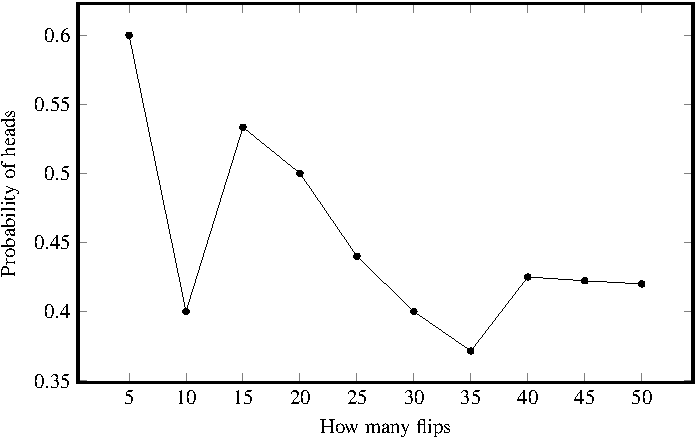
\includegraphics[scale=1]{image/07/coin-flip-scatterplot.pdf}
\caption{%%
  A scatter plot of the data in
  \Table{tab:coin_flip_probability_heads}.
}
\label{fig:coin_flip_scatter_plot}
\end{figure}
\end{solution}
}{}
\end{problem}

\end{document}
